\documentclass[12pt]{article}
\usepackage[T1]{fontenc}
\usepackage[T1]{polski}
\usepackage[utf8]{inputenc}
\newcommand{\BibTeX}{{\sc Bib}\TeX}
\usepackage{graphicx}
\usepackage{amsfonts}

% OWN PACKAGE - VERY IMPORTANT %
\usepackage{float}
%%%%%%%%%%%%%%%%%%%%%%%%%%%%%%%%%

\setlength{\textheight}{21cm}


\title{{\bf Zadanie nr 2 - Próbkowanie i kwantyzacja}\linebreak
    Cyfrowe Przetwarzanie Sygnałów}
\author{Jan Karwowski 216793 \and Kamil Kowalewski 216806}
\date{data oddania zadania 22.04.2020r}

\begin{document}
    \clearpage\maketitle
    \thispagestyle{empty}
    \newpage
    \setcounter{page}{1}
%--------------------------------------------------------------------------------------%
    \section{Cel zadania} {
        Celem zadania jest zapoznanie się z praktycznymi aspektami procesu konwersji
        analogowo-cyfrowej (A/C) i cyfrowo-analogowej (C/A) sygnałów oraz na zaimplementowaniu
        w programie z zadania pierwszego procesu konwersji analogowo-cyfrowej z uwzględnieniem
        operacji próbkowania i kwantyzacji oraz konwersji cyfrowo-analogowej.
    }
%--------------------------------------------------------------------------------------%
    \section{Wstęp teoretyczny} {
        Na podstawie instrukcji ze strony przedmiotu do programu z zadania
        pierwszego zostały dodane funkcjonalności do procesu konwersji analogowo-cyfrowej (A/C)
        i cyfrowo-analogowej (C/A) sygnałów. Warto zaznaczyć, że zostały wykonane wszystkie
        dostępne warianty z instrukcji do zadania i zostały one przedstawione poniżej:

        \begin{itemize}
            \item {Konwersja A/C - próbkowanie}
            \begin{itemize}
                \item (S1) Próbkowanie równomierne
            \end{itemize}

            \item {Konwersja A/C - kwantyzacja}
            \begin{itemize}
                \item (Q1) Kwantyzacja równomierna z obcięciem
                \item (Q2) Kwantyzacja równomierna z zaokrąglaniem
            \end{itemize}

            \item {Konwersja C/A - rekonstrukcja sygnału}
            \begin{itemize}
                \item (R1) Ekstrapolacja zerowego rzędu
                \item (R2) Interpolacja pierwszego rzędu
                \item (R3) Rekonstrukcja w oparciu o funkcję sinc
            \end{itemize}
        \end{itemize}

        Co więcej należało zaimplementować miary, które służą do oceny zrekonstrułowanego
        sygnału z oryginalnym na podstawie porównania częstotliwości próbkowania i progu
        kwantyzacji oraz wyboru metody interpolacji. Miary zostały przedstawione poniżej:
        \begin{itemize}
            \item {
                (C1) Błąd średniokwadratowy (MSE):
                \begin{figure}[H]
                    \centering
                    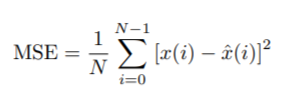
\includegraphics[width=0.4\textwidth]{img/theory/blad-sredniokwad.png}
                \end{figure}
            }
            \item {
                (C2) Stosunek sygnał - szum (SNR):
                \begin{figure}[H]
                    \centering
                    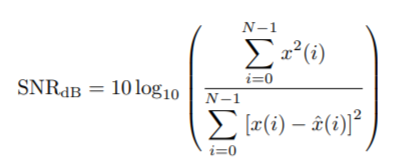
\includegraphics[width=0.4\textwidth]{img/theory/stos-sygn-szum.png}
                \end{figure}
            }
            \item {
                (C3) Szczytowy stosunek sygnał - szum (PSNR):
                \begin{figure}[H]
                    \centering
                    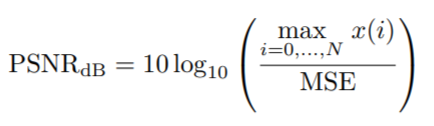
\includegraphics[width=0.4\textwidth]{img/theory/szyt-stos-sygn-szum.png}
                \end{figure}
            }
            \item {
                (C4) Maksymalna różnica (MD):
                \begin{figure}[H]
                    \centering
                    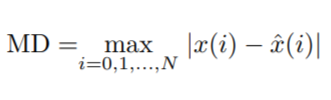
\includegraphics[width=0.4\textwidth]{img/theory/max-roznica.png}
                \end{figure}
            }
            \item {
                Efektywna liczba bitów (ENOB)
            }
        \end{itemize}
    }
    \newpage
%--------------------------------------------------------------------------------------%
    \section{Materiały i metody} {
        Pojedyńczy eksperyment składał się z kilku kroków. W przypadku badania jakości
        rekonstrukcji sygnału wykonywaliśmy generowanie sygnału, następnie jego próbkowanie,
        następnie jego rekonstrukcje i porównanie sygnału pierwotnego z uzyskanym po rekonstrukcji.
        W kolejnym kroku rysowaliśmy na jednym wykresie dwa w/w sygnały. Dla badania kwantyzacji
        kroki były analogiczne z tą różnicą, że krok rekonstrukcji był zastępowany przez
        kwantyzację. Program był uruchmiany ze stosownymi parametrami poprzez skypt w języku
        Python. Kolorem czerwonym został oznaczony sygnał pierwotny natomiast kolorem pomarańczowym
        sygnał po rekonstrukcji lub kwantyzacji zależnie od przeprowadzanego eksperymentu.\\\\

        W tabeli dla parametrów wejściowych przyjeliśmy oznaczenia numeryczne: sygnał - [1],
        czas trwania sygnału - [2], częstotliwość sygnału - [3], częstotliwość próbkowania[4],
        metoda rekonstrukcji(dla sinc również wartość parametru N) / liczba poziomów kwantyzacji - [5]. \\\\

        W tabeli dla parametrów wyjściowych przyjeliśmy następujące oznaczenia numeryczne:
        Błąd średniokwadratowy - [1], Stosunek sygnał - szum - [2],
        Szczytowy stosunek sygnał - szum - [3], Maksymalna różnica - [4], dodatkowo dla badania kwantyzacji
        Teoretyczny stosunek sygnał - szum - [5], Efektywna liczba bitów - [6]
    }
    \newpage
%--------------------------------------------------------------------------------------%
    \section{Eksperymenty i wyniki} {

        \subsection{Badanie jakości rekonstrukcji sygnału - Wpływ zależności między częstotliwością
        sygnału a częstotliwością próbkowania na jakość rekonstrukcji dla jej różnych rodzajów} {

            \subsubsection{Eksperyment 1} {
                \begin{table}[H]
                    \centering
                    \begin{tabular}{|l|l|l|l|l|}
                        \hline
                        1 & 2 & 3 & 4 & 5   \\ \hline
                        sin & 0.5 & 0.1 & 21 & sinc 100    \\ \hline
                    \end{tabular}
                    \caption{Parametry wejściowe}
                \end{table}

                \begin{table}[H]
                    \centering
                    \begin{tabular}{|l|l|l|l|l|}
                        \hline
                        1 & 2 & 3 & 4   \\ \hline
                        0,7406 & -3,3786 & 2,3782 & 2,1861 \\ \hline
                    \end{tabular}
                    \caption{Parametry wyjściowe}
                \end{table}


                \begin{figure}[H]
                    \centering
                    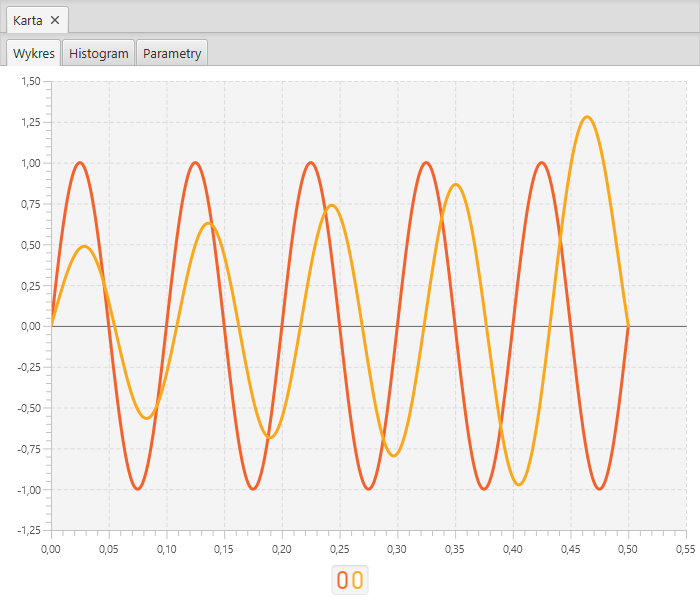
\includegraphics[width=0.8\textwidth]{img/result/experiment1/01/data_draw_original_chart_recon_output_130101.png}
                    \caption{Wykres sygnałów}
                \end{figure}
            }
            \newpage

            \subsubsection{Eksperyment 2} {
                \begin{table}[H]
                    \centering
                    \begin{tabular}{|l|l|l|l|l|}
                        \hline
                        1 & 2 & 3 & 4 & 5   \\ \hline
                        sin & 0.5 & 0.1 & 30 & sinc 100    \\ \hline
                    \end{tabular}
                    \caption{Parametry wejściowe}
                \end{table}

                \begin{table}[H]
                    \centering
                    \begin{tabular}{|l|l|l|l|l|}
                        \hline
                        1 & 2 & 3 & 4   \\ \hline
                        0,0044 & 20,5056 & 23,8418 & 0,2105  \\ \hline
                    \end{tabular}
                    \caption{Parametry wyjściowe}
                \end{table}


                \begin{figure}[H]
                    \centering
                    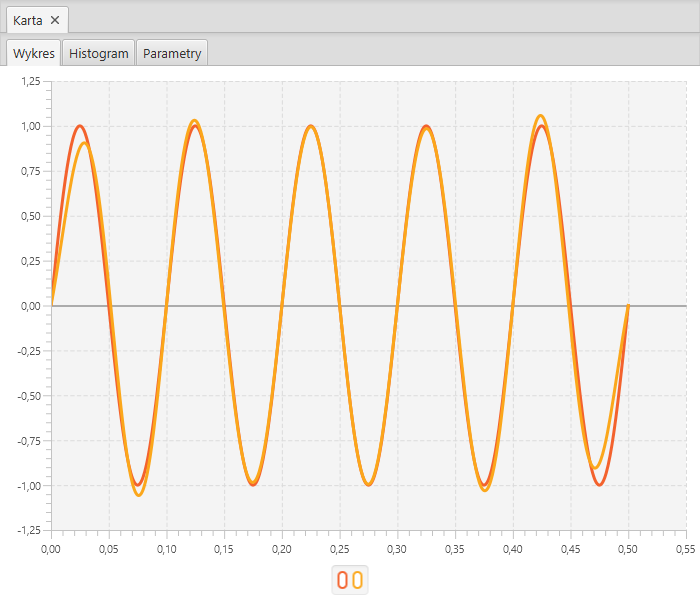
\includegraphics[width=0.8\textwidth]{img/result/experiment1/02/data_draw_original_chart_recon_output_130117.png}
                    \caption{Wykres sygnałów}
                \end{figure}
            }
            \newpage

            \subsubsection{Eksperyment 3} {
                \begin{table}[H]
                    \centering
                    \begin{tabular}{|l|l|l|l|l|}
                        \hline
                        1 & 2 & 3 & 4 & 5   \\ \hline
                        sin & 0.5 & 0.1 & 50 & sinc 100   \\ \hline
                    \end{tabular}
                    \caption{Parametry wejściowe}
                \end{table}

                \begin{table}[H]
                    \centering
                    \begin{tabular}{|l|l|l|l|l|}
                        \hline
                        1 & 2 & 3 & 4   \\ \hline
                        0,0008 & 27,7767 & 31,0143 & 0,1203   \\ \hline
                    \end{tabular}
                    \caption{Parametry wyjściowe}
                \end{table}


                \begin{figure}[H]
                    \centering
                    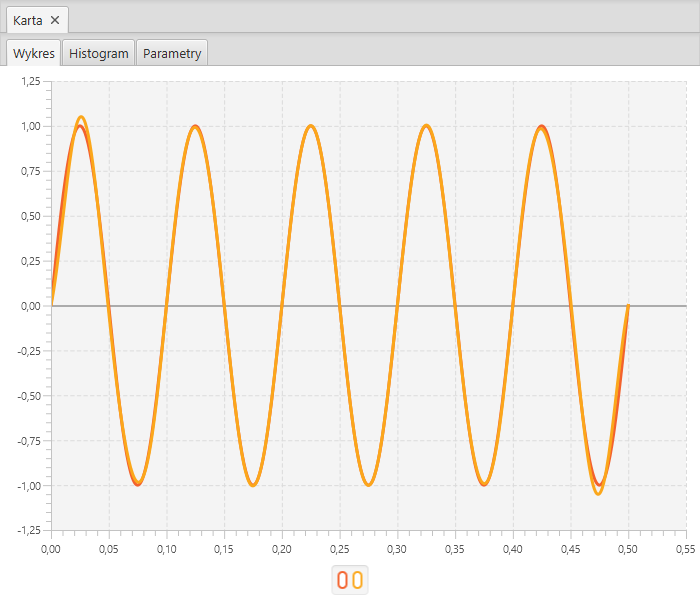
\includegraphics[width=0.8\textwidth]{img/result/experiment1/03/data_draw_original_chart_recon_output_130136.png}
                    \caption{Wykres sygnałów}
                \end{figure}
            }
            \newpage

            \subsubsection{Eksperyment 4} {
                \begin{table}[H]
                    \centering
                    \begin{tabular}{|l|l|l|l|l|}
                        \hline
                        1 & 2 & 3 & 4 & 5   \\ \hline
                        sin & 0.5 & 0.1 & 100 & sinc 100  \\ \hline
                    \end{tabular}
                    \caption{Parametry wejściowe}
                \end{table}

                \begin{table}[H]
                    \centering
                    \begin{tabular}{|l|l|l|l|l|}
                        \hline
                        1 & 2 & 3 & 4   \\ \hline
                        0,0001 & 36,0595 & 39,0525 & 0,0613   \\ \hline
                    \end{tabular}
                    \caption{Parametry wyjściowe}
                \end{table}


                \begin{figure}[H]
                    \centering
                    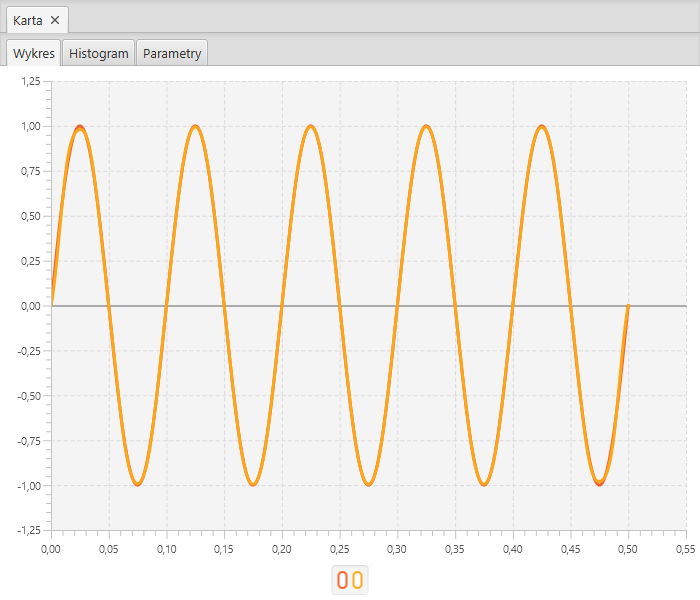
\includegraphics[width=0.8\textwidth]{img/result/experiment1/04/data_draw_original_chart_recon_output_130204.png}
                    \caption{Wykres sygnałów}
                \end{figure}
            }
            \newpage

            \subsubsection{Eksperyment 5} {
                \begin{table}[H]
                    \centering
                    \begin{tabular}{|l|l|l|l|l|}
                        \hline
                        1 & 2 & 3 & 4 & 5   \\ \hline
                        sin & 0.5 & 0.1 & 30 & zero\_order   \\ \hline
                    \end{tabular}
                    \caption{Parametry wejściowe}
                \end{table}

                \begin{table}[H]
                    \centering
                    \begin{tabular}{|l|l|l|l|l|}
                        \hline
                        1 & 2 & 3 & 4   \\ \hline
                        0,5865 & -0,693 & 1,6926 & 1,732   \\ \hline
                    \end{tabular}
                    \caption{Parametry wyjściowe}
                \end{table}


                \begin{figure}[H]
                    \centering
                    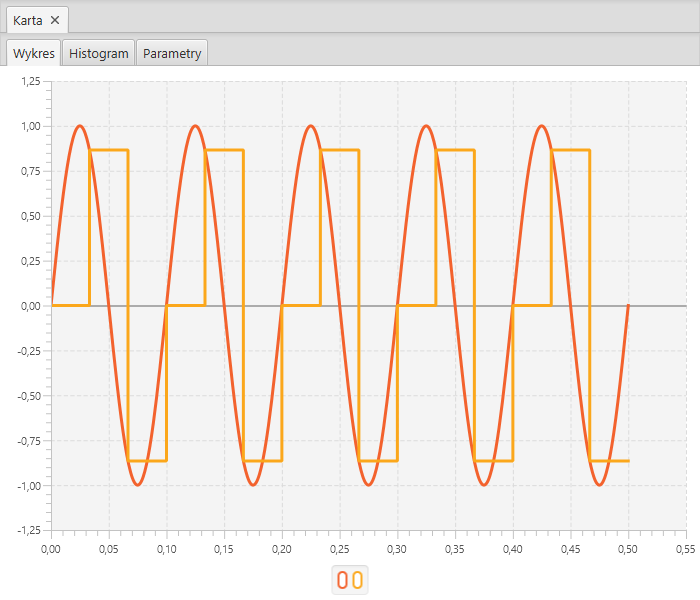
\includegraphics[width=0.8\textwidth]{img/result/experiment1/05/data_draw_original_chart_recon_output_130214.png}
                    \caption{Wykres sygnałów}
                \end{figure}
            }
            \newpage

            \subsubsection{Eksperyment 6} {
                \begin{table}[H]
                    \centering
                    \begin{tabular}{|l|l|l|l|l|}
                        \hline
                        1 & 2 & 3 & 4 & 5   \\ \hline
                        sin & 0.5 & 0.1 & 50 & zero\_order    \\ \hline
                    \end{tabular}
                    \caption{Parametry wejściowe}
                \end{table}

                \begin{table}[H]
                    \centering
                    \begin{tabular}{|l|l|l|l|l|}
                        \hline
                        1 & 2 & 3 & 4   \\ \hline
                        0,2432 & 3,1307 & 5,9231 & 1,1755   \\ \hline
                    \end{tabular}
                    \caption{Parametry wyjściowe}
                \end{table}


                \begin{figure}[H]
                    \centering
                    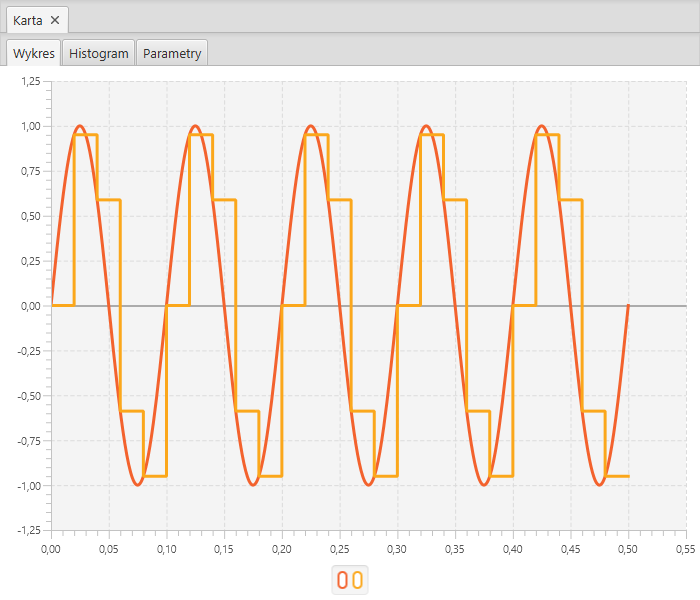
\includegraphics[width=0.8\textwidth]{img/result/experiment1/06/data_draw_original_chart_recon_output_130225.png}
                    \caption{Wykres sygnałów}
                \end{figure}
            }
            \newpage

            \subsubsection{Eksperyment 7} {
                \begin{table}[H]
                    \centering
                    \begin{tabular}{|l|l|l|l|l|}
                        \hline
                        1 & 2 & 3 & 4 & 5   \\ \hline
                        sin & 0.5 & 0.1 & 100 & zero\_order   \\ \hline
                    \end{tabular}
                    \caption{Parametry wejściowe}
                \end{table}

                \begin{table}[H]
                    \centering
                    \begin{tabular}{|l|l|l|l|l|}
                        \hline
                        1 & 2 & 3 & 4   \\ \hline
                        0,0645 & 8,8936 & 11,686 & 0,5878   \\ \hline
                    \end{tabular}
                    \caption{Parametry wyjściowe}
                \end{table}


                \begin{figure}[H]
                    \centering
                    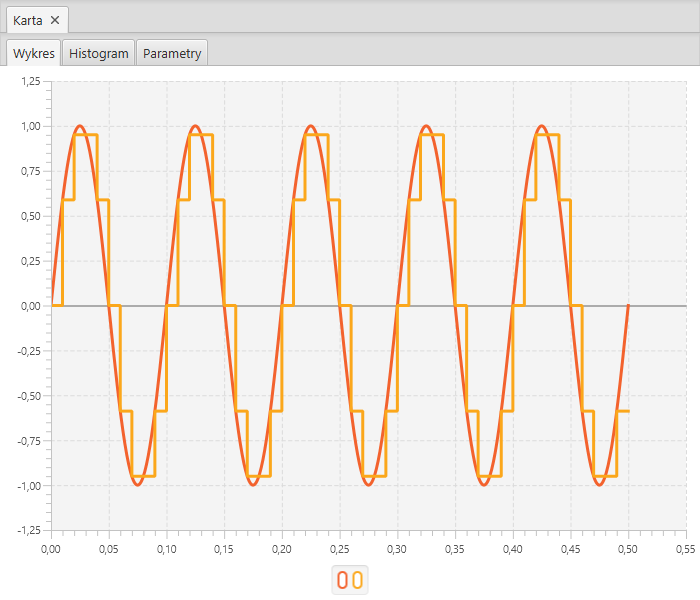
\includegraphics[width=0.8\textwidth]{img/result/experiment1/07/data_draw_original_chart_recon_output_130235.png}
                    \caption{Wykres sygnałów}
                \end{figure}
            }
            \newpage

            \subsubsection{Eksperyment 8} {
                \begin{table}[H]
                    \centering
                    \begin{tabular}{|l|l|l|l|l|}
                        \hline
                        1 & 2 & 3 & 4 & 5   \\ \hline
                        sin & 0.5 & 0.1 & 30 & first\_order   \\ \hline
                    \end{tabular}
                    \caption{Parametry wejściowe}
                \end{table}

                \begin{table}[H]
                    \centering
                    \begin{tabular}{|l|l|l|l|l|}
                        \hline
                        1 & 2 & 3 & 4   \\ \hline
                        0,0671 & 6,2571 & 11,1094 & 0,866  \\ \hline
                    \end{tabular}
                    \caption{Parametry wyjściowe}
                \end{table}


                \begin{figure}[H]
                    \centering
                    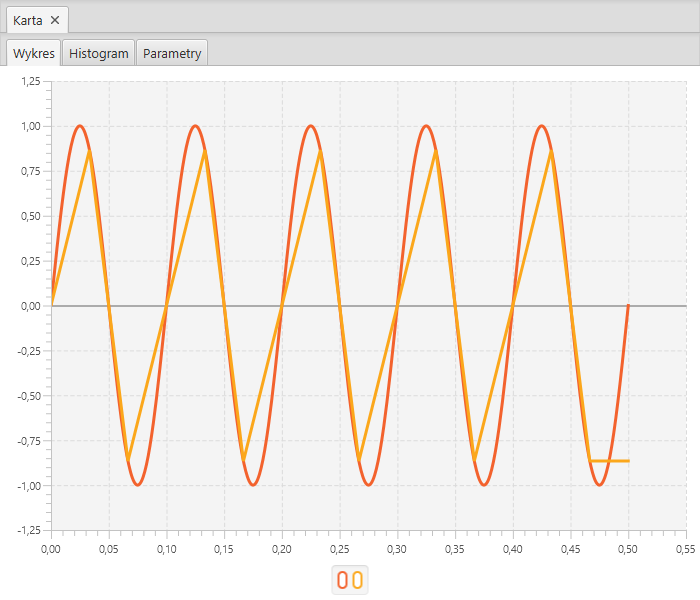
\includegraphics[width=0.8\textwidth]{img/result/experiment1/08/data_draw_original_chart_recon_output_130245.png}
                    \caption{Wykres sygnałów}
                \end{figure}
            }
            \newpage

            \subsubsection{Eksperyment 9} {
                \begin{table}[H]
                    \centering
                    \begin{tabular}{|l|l|l|l|l|}
                        \hline
                        1 & 2 & 3 & 4 & 5   \\ \hline
                        sin & 0.5 & 0.1 & 50 & first\_order   \\ \hline
                    \end{tabular}
                    \caption{Parametry wejściowe}
                \end{table}

                \begin{table}[H]
                    \centering
                    \begin{tabular}{|l|l|l|l|l|}
                        \hline
                        1 & 2 & 3 & 4   \\ \hline
                        0,0191 & 13,3081 & 16,9734 & 0,951  \\ \hline
                    \end{tabular}
                    \caption{Parametry wyjściowe}
                \end{table}


                \begin{figure}[H]
                    \centering
                    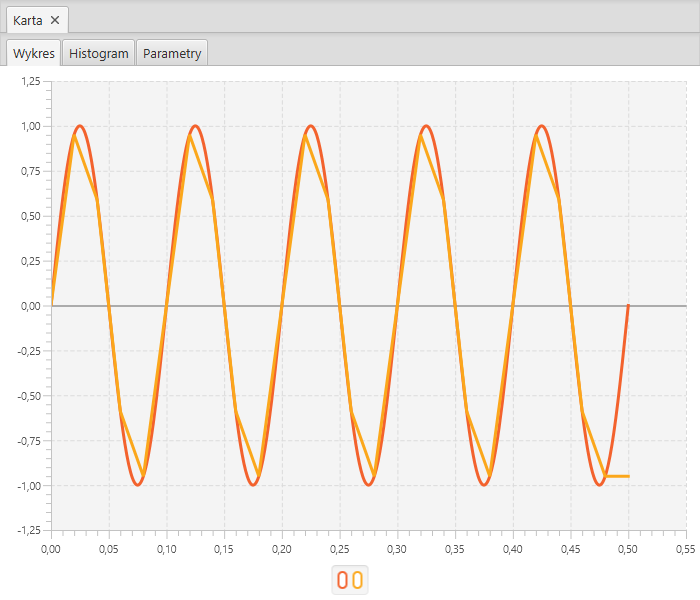
\includegraphics[width=0.8\textwidth]{img/result/experiment1/09/data_draw_original_chart_recon_output_130256.png}
                    \caption{Wykres sygnałów}
                \end{figure}
            }
            \newpage

            \subsubsection{Eksperyment 10} {
                \begin{table}[H]
                    \centering
                    \begin{tabular}{|l|l|l|l|l|}
                        \hline
                        1 & 2 & 3 & 4 & 5   \\ \hline
                        sin & 0.5 & 0.1 & 100 & first\_order  \\ \hline
                    \end{tabular}
                    \caption{Parametry wejściowe}
                \end{table}

                \begin{table}[H]
                    \centering
                    \begin{tabular}{|l|l|l|l|l|}
                        \hline
                        1 & 2 & 3 & 4   \\ \hline
                        0,0028 & 22,2276 & 25,2631 & 0,5878  \\ \hline
                    \end{tabular}
                    \caption{Parametry wyjściowe}
                \end{table}


                \begin{figure}[H]
                    \centering
                    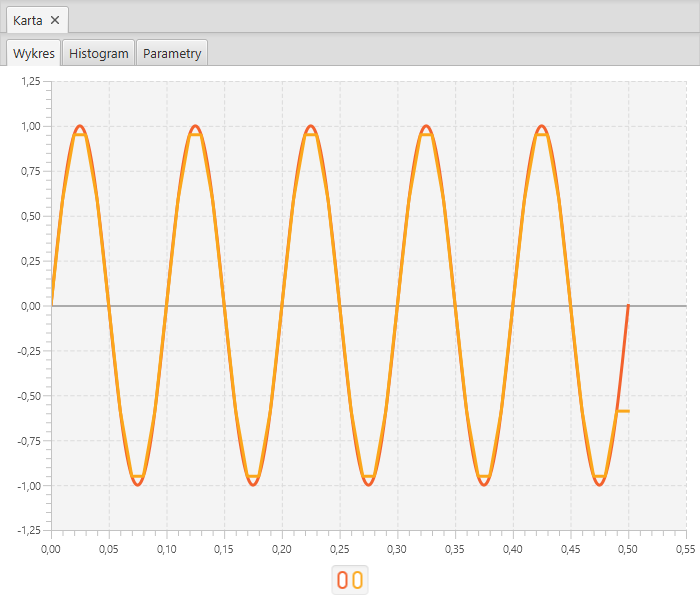
\includegraphics[width=0.8\textwidth]{img/result/experiment1/10/data_draw_original_chart_recon_output_130307.png}
                    \caption{Wykres sygnałów}
                \end{figure}
            }
        }

        \subsection{Badanie jakości rekonstrukcji sygnału - Wpływ rodzaju sygnału na jakość
        rekonstrukcji dla jej różnych rodzajów} {

            \subsubsection{Eksperyment 1} {
                \begin{table}[H]
                    \centering
                    \begin{tabular}{|l|l|l|l|l|}
                        \hline
                        1 & 2 & 3 & 4 & 5   \\ \hline
                        sin & 0.5 & 0.1 & 50 & sinc 100  \\ \hline
                    \end{tabular}
                    \caption{Parametry wejściowe}
                \end{table}

                \begin{table}[H]
                    \centering
                    \begin{tabular}{|l|l|l|l|l|}
                        \hline
                        1 & 2 & 3 & 4   \\ \hline
                        0,0008 & 27,7767 & 31,0143 & 0,1203 \\ \hline
                    \end{tabular}
                    \caption{Parametry wyjściowe}
                \end{table}


                \begin{figure}[H]
                    \centering
                    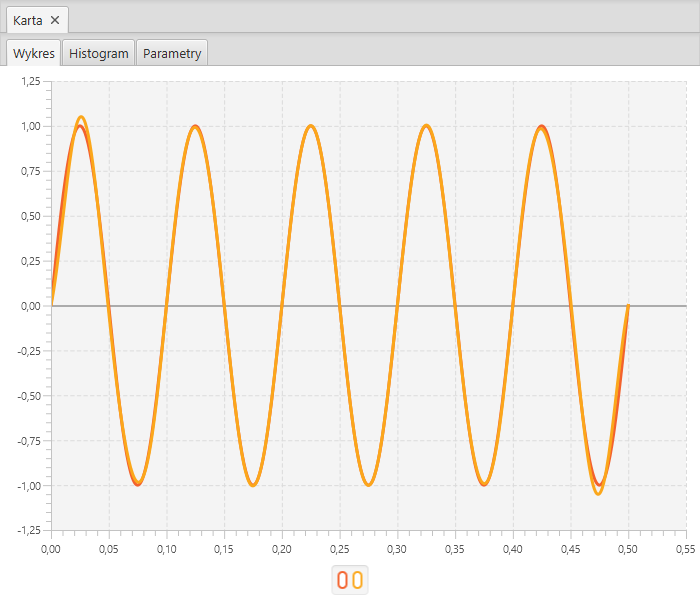
\includegraphics[width=0.8\textwidth]{img/result/experiment2/01/data_draw_original_chart_recon_output_130327.png}
                    \caption{Wykres sygnałów}
                \end{figure}
            }
            \newpage

            \subsubsection{Eksperyment 2} {
                \begin{table}[H]
                    \centering
                    \begin{tabular}{|l|l|l|l|l|}
                        \hline
                        1 & 2 & 3 & 4 & 5   \\ \hline
                        rect & 0.5 & 0.1 & 50 & sinc 100  \\ \hline
                    \end{tabular}
                    \caption{Parametry wejściowe}
                \end{table}

                \begin{table}[H]
                    \centering
                    \begin{tabular}{|l|l|l|l|l|}
                        \hline
                        1 & 2 & 3 & 4   \\ \hline
                        0,0898 & 7,8085 & 11,4253 & 1  \\ \hline
                    \end{tabular}
                    \caption{Parametry wyjściowe}
                \end{table}


                \begin{figure}[H]
                    \centering
                    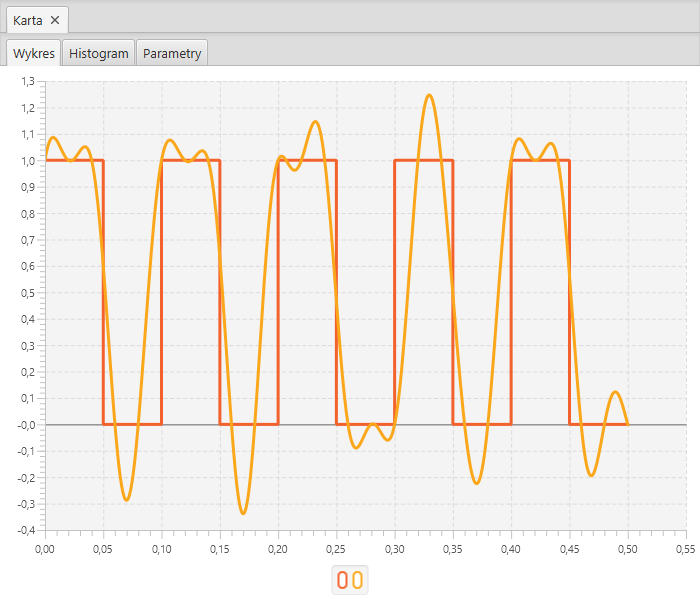
\includegraphics[width=0.8\textwidth]{img/result/experiment2/02/data_draw_original_chart_recon_output_130343.png}
                    \caption{Wykres sygnałów}
                \end{figure}
            }
            \newpage

            \subsubsection{Eksperyment 3} {
                \begin{table}[H]
                    \centering
                    \begin{tabular}{|l|l|l|l|l|}
                        \hline
                        1 & 2 & 3 & 4 & 5   \\ \hline
                        triang & 0.5 & 0.1 & 50 & sinc 100    \\ \hline
                    \end{tabular}
                    \caption{Parametry wejściowe}
                \end{table}

                \begin{table}[H]
                    \centering
                    \begin{tabular}{|l|l|l|l|l|}
                        \hline
                        1 & 2 & 3 & 4   \\ \hline
                        0,0033 & 19,8458 & 24,0553 & 0,1634 \\ \hline
                    \end{tabular}
                    \caption{Parametry wyjściowe}
                \end{table}


                \begin{figure}[H]
                    \centering
                    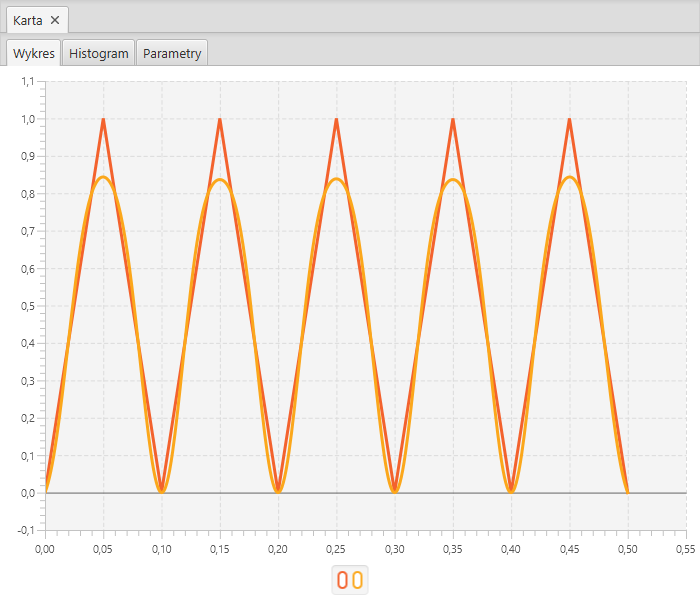
\includegraphics[width=0.8\textwidth]{img/result/experiment2/03/data_draw_original_chart_recon_output_130358.png}
                    \caption{Wykres sygnałów}
                \end{figure}
            }
            \newpage

            \subsubsection{Eksperyment 4} {
                \begin{table}[H]
                    \centering
                    \begin{tabular}{|l|l|l|l|l|}
                        \hline
                        1 & 2 & 3 & 4 & 5   \\ \hline
                        sin & 0.5 & 0.1 & 50 & zero\_order  \\ \hline
                    \end{tabular}
                    \caption{Parametry wejściowe}
                \end{table}

                \begin{table}[H]
                    \centering
                    \begin{tabular}{|l|l|l|l|l|}
                        \hline
                        1 & 2 & 3 & 4   \\ \hline
                        0,2432 & 3,1307 & 5,9231 & 1,1755 \\ \hline
                    \end{tabular}
                    \caption{Parametry wyjściowe}
                \end{table}


                \begin{figure}[H]
                    \centering
                    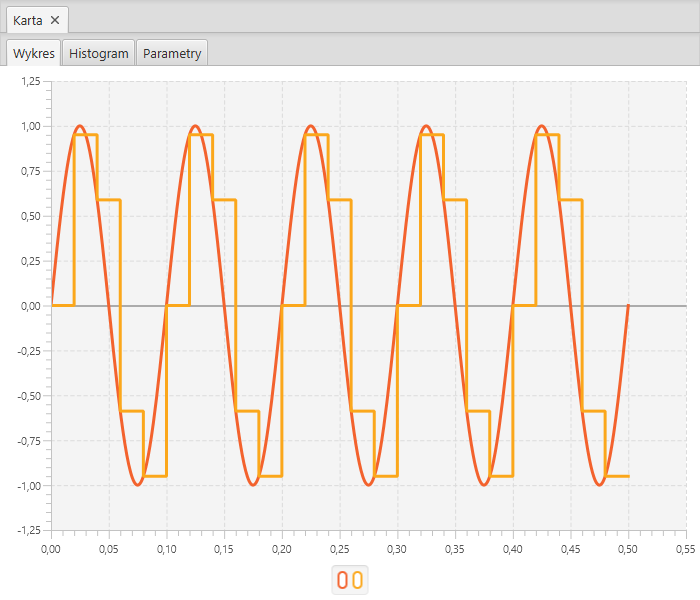
\includegraphics[width=0.8\textwidth]{img/result/experiment2/04/data_draw_original_chart_recon_output_130409.png}
                    \caption{Wykres sygnałów}
                \end{figure}
            }
            \newpage

            \subsubsection{Eksperyment 5} {
                \begin{table}[H]
                    \centering
                    \begin{tabular}{|l|l|l|l|l|}
                        \hline
                        1 & 2 & 3 & 4 & 5   \\ \hline
                        rect & 0.5 & 0.1 & 50 & zero\_order  \\ \hline
                    \end{tabular}
                    \caption{Parametry wejściowe}
                \end{table}

                \begin{table}[H]
                    \centering
                    \begin{tabular}{|l|l|l|l|l|}
                        \hline
                        1 & 2 & 3 & 4   \\ \hline
                        0,14 & 6,0207 & 8,5388 & 1 \\ \hline
                    \end{tabular}
                    \caption{Parametry wyjściowe}
                \end{table}


                \begin{figure}[H]
                    \centering
                    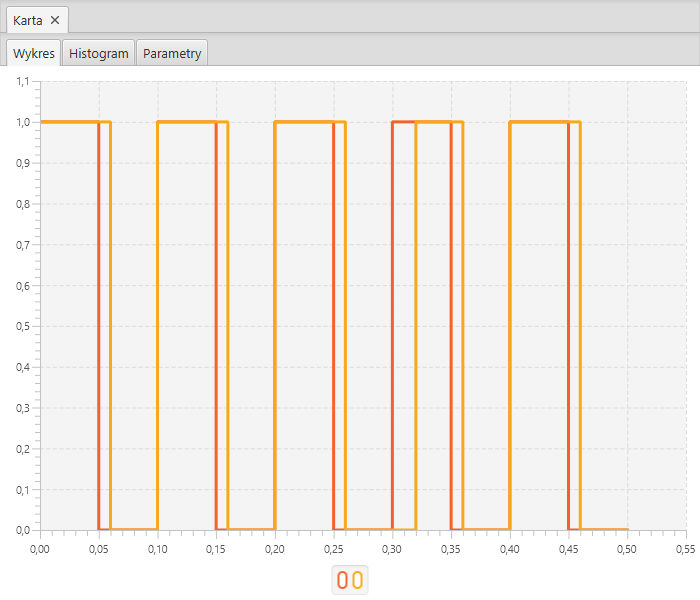
\includegraphics[width=0.8\textwidth]{img/result/experiment2/05/data_draw_original_chart_recon_output_130418.png}
                    \caption{Wykres sygnałów}
                \end{figure}
            }
            \newpage

            \subsubsection{Eksperyment 6} {
                \begin{table}[H]
                    \centering
                    \begin{tabular}{|l|l|l|l|l|}
                        \hline
                        1 & 2 & 3 & 4 & 5   \\ \hline
                        triang &0.5 & 0.1 & 50 & zero\_order  \\ \hline
                    \end{tabular}
                    \caption{Parametry wejściowe}
                \end{table}

                \begin{table}[H]
                    \centering
                    \begin{tabular}{|l|l|l|l|l|}
                        \hline
                        1 & 2 & 3 & 4   \\ \hline
                        0,0453 & 8,4874 & 12,4668 & 0,4 \\ \hline
                    \end{tabular}
                    \caption{Parametry wyjściowe}
                \end{table}


                \begin{figure}[H]
                    \centering
                    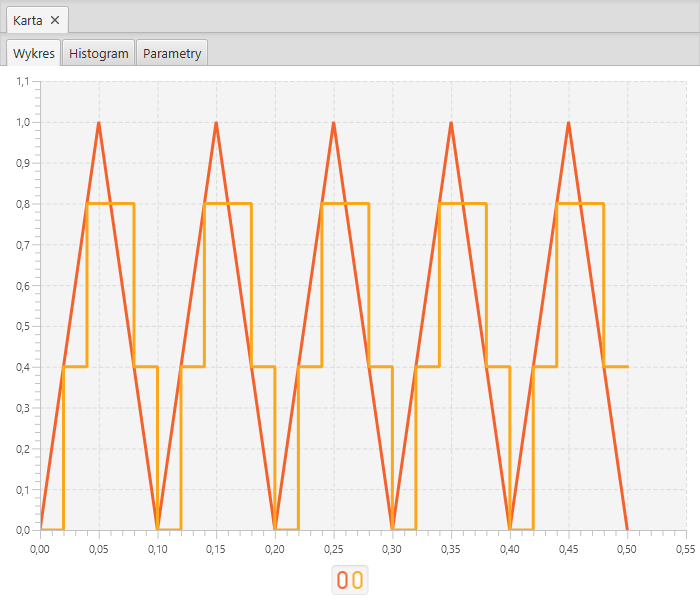
\includegraphics[width=0.8\textwidth]{img/result/experiment2/06/data_draw_original_chart_recon_output_130428.png}
                    \caption{Wykres sygnałów}
                \end{figure}
            }
            \newpage

            \subsubsection{Eksperyment 7} {
                \begin{table}[H]
                    \centering
                    \begin{tabular}{|l|l|l|l|l|}
                        \hline
                        1 & 2 & 3 & 4 & 5   \\ \hline
                        sin & 0.5 & 0.1 & 50 & first\_order  \\ \hline
                    \end{tabular}
                    \caption{Parametry wejściowe}
                \end{table}

                \begin{table}[H]
                    \centering
                    \begin{tabular}{|l|l|l|l|l|}
                        \hline
                        1 & 2 & 3 & 4   \\ \hline
                        0,0191 & 13,3081 & 16,9734 & 0,951 \\ \hline
                    \end{tabular}
                    \caption{Parametry wyjściowe}
                \end{table}


                \begin{figure}[H]
                    \centering
                    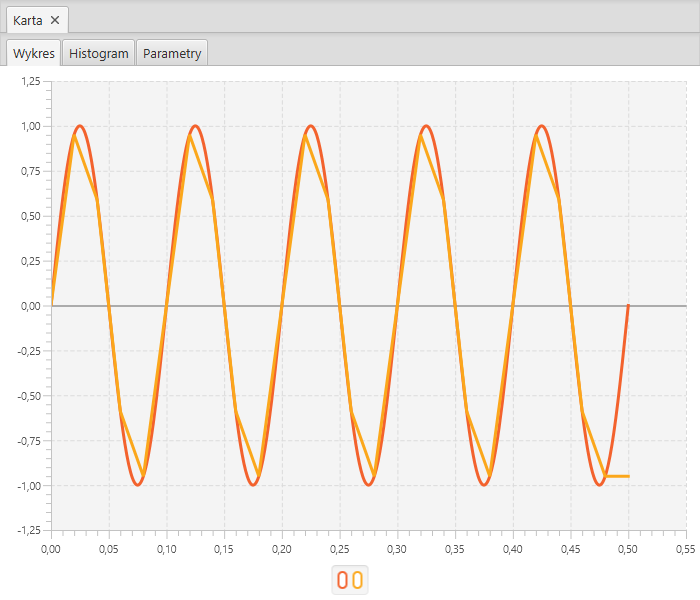
\includegraphics[width=0.8\textwidth]{img/result/experiment2/07/data_draw_original_chart_recon_output_130439.png}
                    \caption{Wykres sygnałów}
                \end{figure}
            }
            \newpage

            \subsubsection{Eksperyment 8} {
                \begin{table}[H]
                    \centering
                    \begin{tabular}{|l|l|l|l|l|}
                        \hline
                        1 & 2 & 3 & 4 & 5   \\ \hline
                        rect & 0.5 & 0.1 & 50 & first\_order  \\ \hline
                    \end{tabular}
                    \caption{Parametry wejściowe}
                \end{table}

                \begin{table}[H]
                    \centering
                    \begin{tabular}{|l|l|l|l|l|}
                        \hline
                        1 & 2 & 3 & 4   \\ \hline
                        0,07 & 8,3614 & 11,549 & 1 \\ \hline
                    \end{tabular}
                    \caption{Parametry wyjściowe}
                \end{table}


                \begin{figure}[H]
                    \centering
                    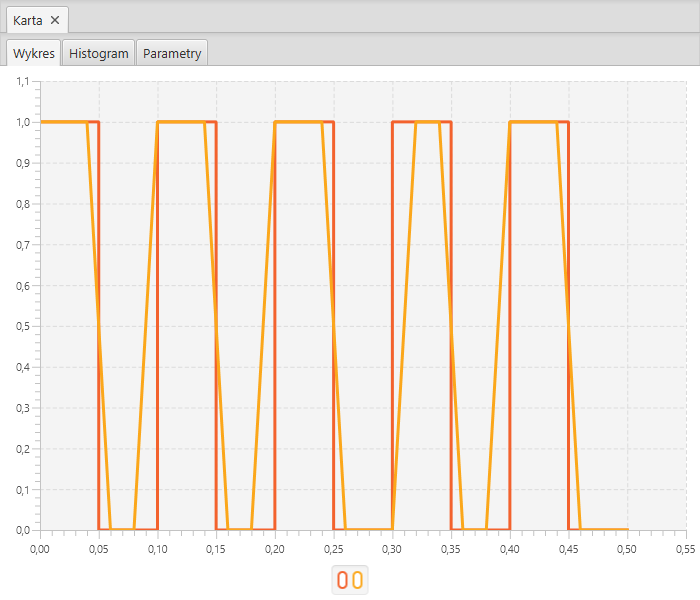
\includegraphics[width=0.8\textwidth]{img/result/experiment2/08/data_draw_original_chart_recon_output_130449.png}
                    \caption{Wykres sygnałów}
                \end{figure}
            }
            \newpage

            \subsubsection{Eksperyment 9} {
                \begin{table}[H]
                    \centering
                    \begin{tabular}{|l|l|l|l|l|}
                        \hline
                        1 & 2 & 3 & 4 & 5   \\ \hline
                        triang & 0.5 & 0.1 & 50 & first\_order   \\ \hline
                    \end{tabular}
                    \caption{Parametry wejściowe}
                \end{table}

                \begin{table}[H]
                    \centering
                    \begin{tabular}{|l|l|l|l|l|}
                        \hline
                        1 & 2 & 3 & 4   \\ \hline
                        0,0048 & 18,0011 & 22,2186 & 0,4 \\ \hline
                    \end{tabular}
                    \caption{Parametry wyjściowe}
                \end{table}


                \begin{figure}[H]
                    \centering
                    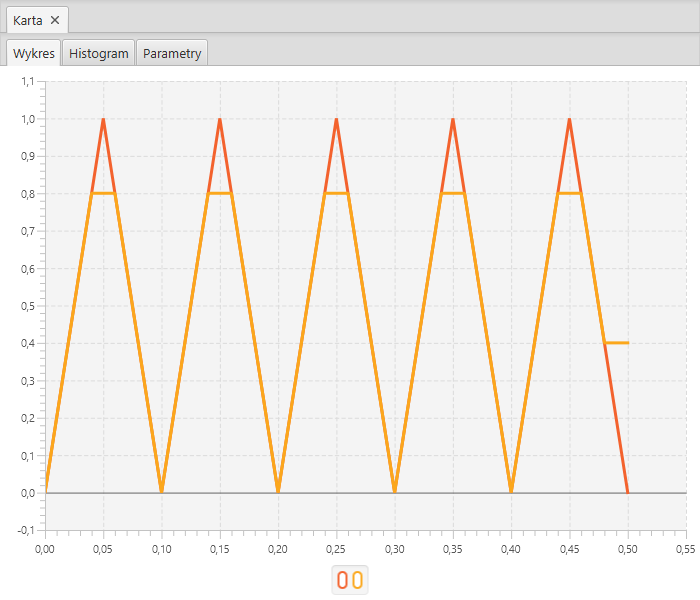
\includegraphics[width=0.8\textwidth]{img/result/experiment2/09/data_draw_original_chart_recon_output_130459.png}
                    \caption{Wykres sygnałów}
                \end{figure}
            }
            \newpage


        }

        \subsection{Badanie jakości rekonstrukcji sygnału - Zjawisko aliasingu} {

            \subsubsection{Eksperyment 1} {
                \begin{table}[H]
                    \centering
                    \begin{tabular}{|l|l|l|l|l|}
                        \hline
                        1 & 2 & 3 & 4 & 5   \\ \hline
                        sin & 1 & 0.143 & 5 & sinc 100   \\ \hline
                    \end{tabular}
                    \caption{Parametry wejściowe}
                \end{table}

                \begin{table}[H]
                    \centering
                    \begin{tabular}{|l|l|l|l|l|}
                        \hline
                        1 & 2 & 3 & 4   \\ \hline
                        0,9123 & -3,4863 & 0,3088 & 1,7882 \\ \hline
                    \end{tabular}
                    \caption{Parametry wyjściowe}
                \end{table}


                \begin{figure}[H]
                    \centering
                    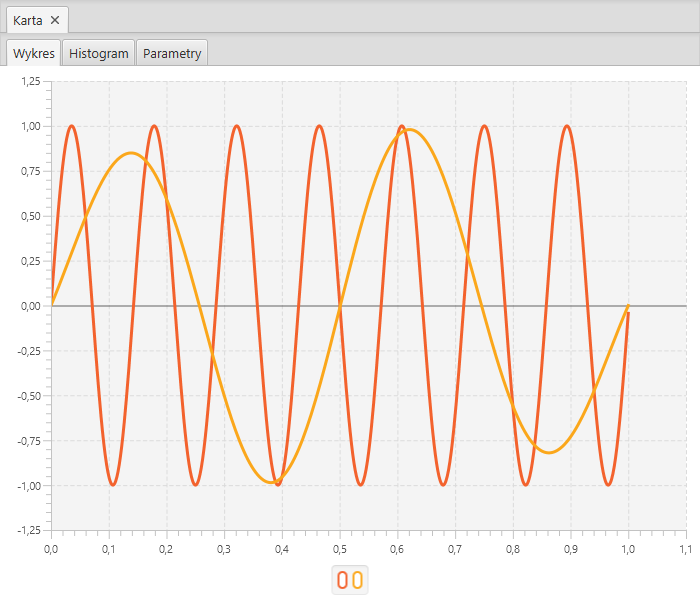
\includegraphics[width=0.8\textwidth]{img/result/experiment3/01/data_draw_original_chart_recon_output_130511.png}
                    \caption{Wykres sygnałów}
                \end{figure}
            }
            \newpage

            \subsubsection{Eksperyment 2} {
                \begin{table}[H]
                    \centering
                    \begin{tabular}{|l|l|l|l|l|}
                        \hline
                        1 & 2 & 3 & 4 & 5   \\ \hline
                        sin & 1 & 0.083 & 5 & sinc 100   \\ \hline
                    \end{tabular}
                    \caption{Parametry wejściowe}
                \end{table}

                \begin{table}[H]
                    \centering
                    \begin{tabular}{|l|l|l|l|l|}
                        \hline
                        1 & 2 & 3 & 4   \\ \hline
                        0,9391 & -3,2786 & 0,2877 & 1,9956 \\ \hline
                    \end{tabular}
                    \caption{Parametry wyjściowe}
                \end{table}


                \begin{figure}[H]
                    \centering
                    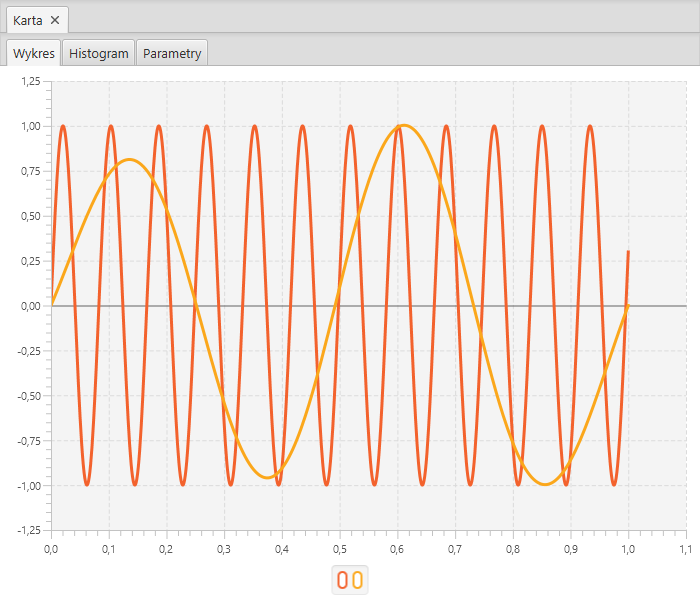
\includegraphics[width=0.8\textwidth]{img/result/experiment3/02/data_draw_original_chart_recon_output_200358.png}
                    \caption{Wykres sygnałów}
                \end{figure}
            }
            \newpage

            \subsubsection{Eksperyment 3} {
                \begin{table}[H]
                    \centering
                    \begin{tabular}{|l|l|l|l|l|}
                        \hline
                        1 & 2 & 3 & 4 & 5   \\ \hline
                        sin & 1 & 0.09 & 5 & sinc 100   \\ \hline
                    \end{tabular}
                    \caption{Parametry wejściowe}
                \end{table}

                \begin{table}[H]
                    \centering
                    \begin{tabular}{|l|l|l|l|l|}
                        \hline
                        1 & 2 & 3 & 4   \\ \hline
                        0,9423 & -3,2491 & 0,4658 & 2,0488 \\ \hline
                    \end{tabular}
                    \caption{Parametry wyjściowe}
                \end{table}


                \begin{figure}[H]
                    \centering
                    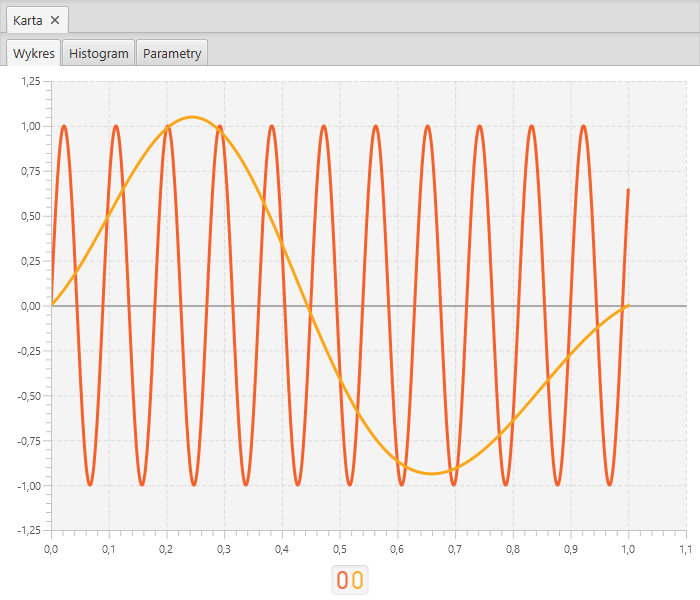
\includegraphics[width=0.8\textwidth]{img/result/experiment3/03/data_draw_original_chart_recon_output_130535.png}
                    \caption{Wykres sygnałów}
                \end{figure}
            }
            \newpage

        }

        \subsection{Badanie jakości rekonstrukcji sygnału - Wpływ wartości N na jakość
        rekonstrukcji przy wykorzystaniu metody sinc} {

            \subsubsection{Eksperyment 1} {
                \begin{table}[H]
                    \centering
                    \begin{tabular}{|l|l|l|l|l|}
                        \hline
                        1 & 2 & 3 & 4 & 5   \\ \hline
                        sin & 0.5 & 0.1 & 50 & sinc 1  \\ \hline
                    \end{tabular}
                    \caption{Parametry wejściowe}
                \end{table}

                \begin{table}[H]
                    \centering
                    \begin{tabular}{|l|l|l|l|l|}
                        \hline
                        1 & 2 & 3 & 4   \\ \hline
                        0,2122 & 0,2682 & 6,5147 & 0,9511 \\ \hline
                    \end{tabular}
                    \caption{Parametry wyjściowe}
                \end{table}


                \begin{figure}[H]
                    \centering
                    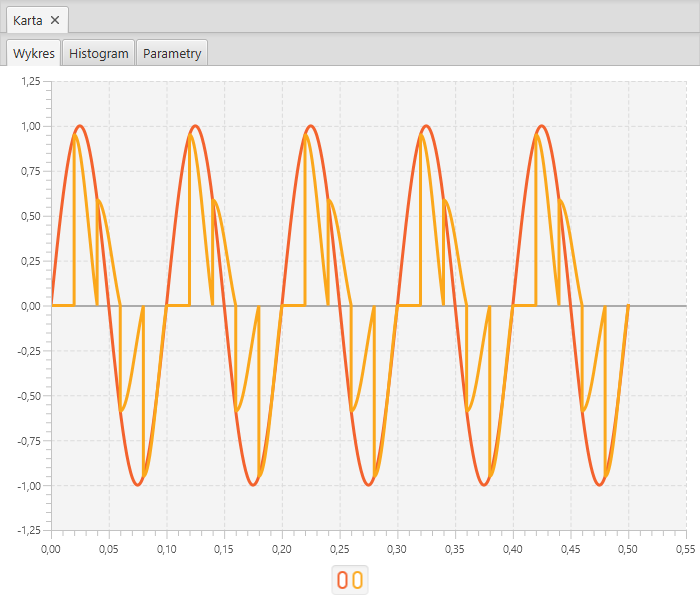
\includegraphics[width=0.8\textwidth]{img/result/experiment4/01/data_draw_original_chart_recon_output_130545.png}
                    \caption{Wykres sygnałów}
                \end{figure}
            }
            \newpage

            \subsubsection{Eksperyment 2} {
                \begin{table}[H]
                    \centering
                    \begin{tabular}{|l|l|l|l|l|}
                        \hline
                        1 & 2 & 3 & 4 & 5   \\ \hline
                        sin & 0.5 & 0.1 & 50 & sinc 2  \\ \hline
                    \end{tabular}
                    \caption{Parametry wejściowe}
                \end{table}

                \begin{table}[H]
                    \centering
                    \begin{tabular}{|l|l|l|l|l|}
                        \hline
                        1 & 2 & 3 & 4   \\ \hline
                        0,15 & 1,7682 & 8,0206 & 0,9511 \\ \hline
                    \end{tabular}
                    \caption{Parametry wyjściowe}
                \end{table}


                \begin{figure}[H]
                    \centering
                    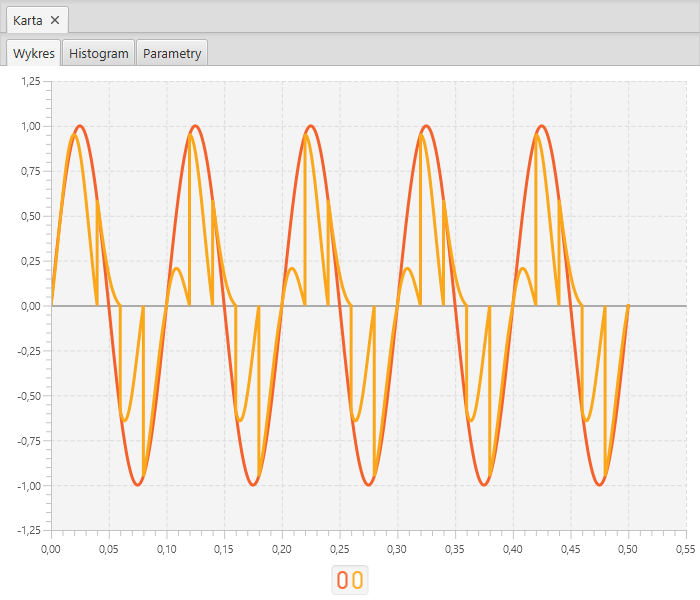
\includegraphics[width=0.8\textwidth]{img/result/experiment4/02/data_draw_original_chart_recon_output_130556.png}
                    \caption{Wykres sygnałów}
                \end{figure}
            }
            \newpage

            \subsubsection{Eksperyment 3} {
                \begin{table}[H]
                    \centering
                    \begin{tabular}{|l|l|l|l|l|}
                        \hline
                        1 & 2 & 3 & 4 & 5   \\ \hline
                        sin & 0.5 & 0.1 & 50 & sinc 3  \\ \hline
                    \end{tabular}
                    \caption{Parametry wejściowe}
                \end{table}

                \begin{table}[H]
                    \centering
                    \begin{tabular}{|l|l|l|l|l|}
                        \hline
                        1 & 2 & 3 & 4   \\ \hline
                        0,0126 & 16,5061 & 19,1377 & 0,2204 \\ \hline
                    \end{tabular}
                    \caption{Parametry wyjściowe}
                \end{table}


                \begin{figure}[H]
                    \centering
                    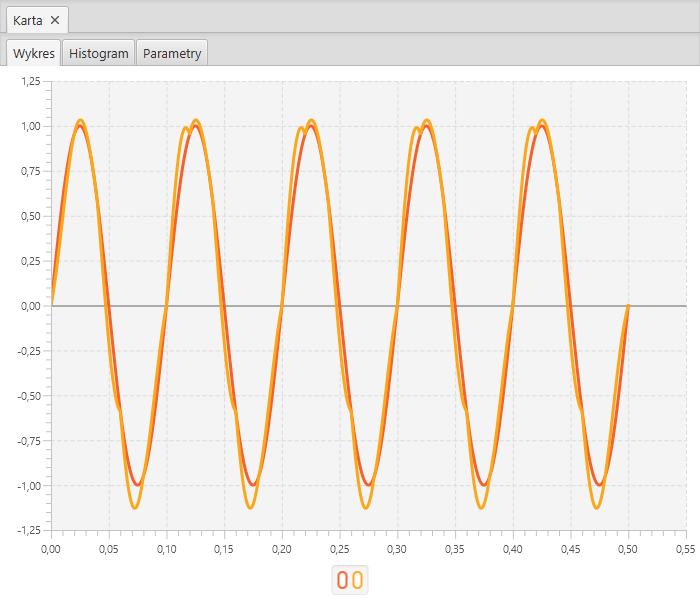
\includegraphics[width=0.8\textwidth]{img/result/experiment4/03/data_draw_original_chart_recon_output_130607.png}
                    \caption{Wykres sygnałów}
                \end{figure}
            }
            \newpage

            \subsubsection{Eksperyment 4} {
                \begin{table}[H]
                    \centering
                    \begin{tabular}{|l|l|l|l|l|}
                        \hline
                        1 & 2 & 3 & 4 & 5   \\ \hline
                        sin & 0.5 & 0.1 & 50 & sinc 4  \\ \hline
                    \end{tabular}
                    \caption{Parametry wejściowe}
                \end{table}

                \begin{table}[H]
                    \centering
                    \begin{tabular}{|l|l|l|l|l|}
                        \hline
                        1 & 2 & 3 & 4   \\ \hline
                        0,0109 & 16,6055 & 20,1448 & 0,2048 \\ \hline
                    \end{tabular}
                    \caption{Parametry wyjściowe}
                \end{table}


                \begin{figure}[H]
                    \centering
                    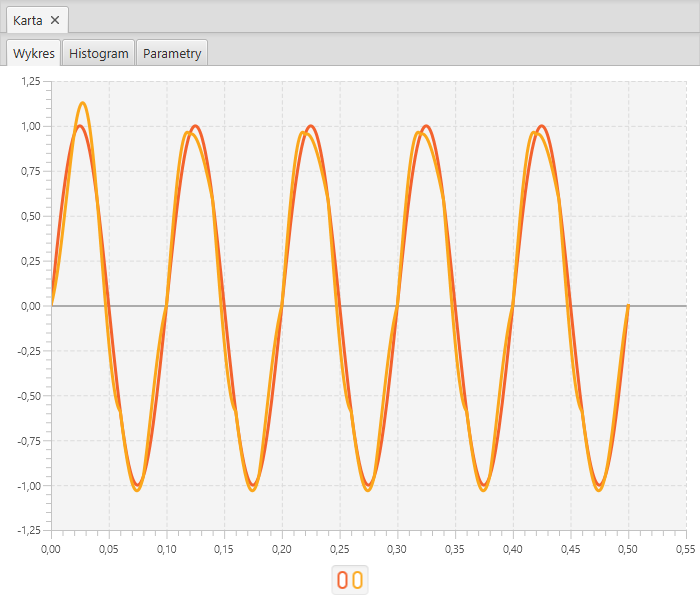
\includegraphics[width=0.8\textwidth]{img/result/experiment4/04/data_draw_original_chart_recon_output_130619.png}
                    \caption{Wykres sygnałów}
                \end{figure}
            }
            \newpage

            \subsubsection{Eksperyment 5} {
                \begin{table}[H]
                    \centering
                    \begin{tabular}{|l|l|l|l|l|}
                        \hline
                        1 & 2 & 3 & 4 & 5   \\ \hline
                        sin & 0.5 & 0.1 & 50 & sinc 5   \\ \hline
                    \end{tabular}
                    \caption{Parametry wejściowe}
                \end{table}

                \begin{table}[H]
                    \centering
                    \begin{tabular}{|l|l|l|l|l|}
                        \hline
                        1 & 2 & 3 & 4   \\ \hline
                        0,0007 & 28,6383 & 31,6574 & 0,1017 \\ \hline
                    \end{tabular}
                    \caption{Parametry wyjściowe}
                \end{table}


                \begin{figure}[H]
                    \centering
                    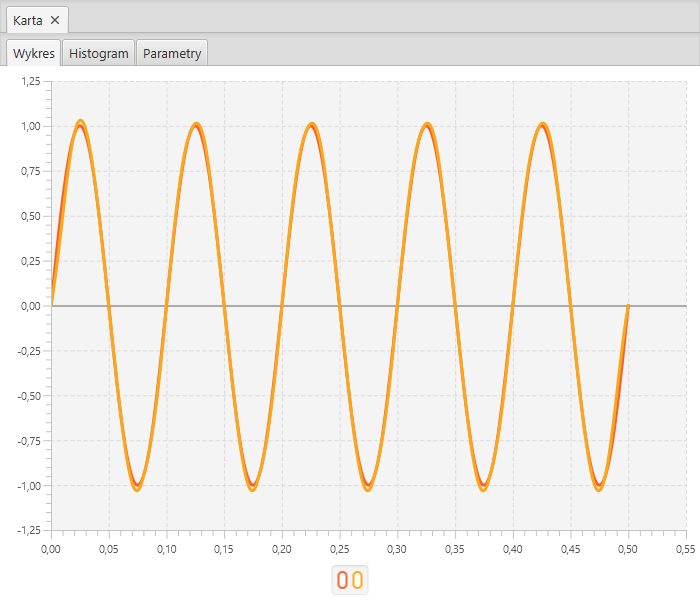
\includegraphics[width=0.8\textwidth]{img/result/experiment4/05/data_draw_original_chart_recon_output_130631.png}
                    \caption{Wykres sygnałów}
                \end{figure}
            }
            \newpage

            \subsubsection{Eksperyment 6} {
                \begin{table}[H]
                    \centering
                    \begin{tabular}{|l|l|l|l|l|}
                        \hline
                        1 & 2 & 3 & 4 & 5   \\ \hline
                        sin & 0.5 & 0.1 & 50 & sinc 10  \\ \hline
                    \end{tabular}
                    \caption{Parametry wejściowe}
                \end{table}

                \begin{table}[H]
                    \centering
                    \begin{tabular}{|l|l|l|l|l|}
                        \hline
                        1 & 2 & 3 & 4   \\ \hline
                        0,0023 & 23,3571 & 26,7293 & 0,1364 \\ \hline
                    \end{tabular}
                    \caption{Parametry wyjściowe}
                \end{table}


                \begin{figure}[H]
                    \centering
                    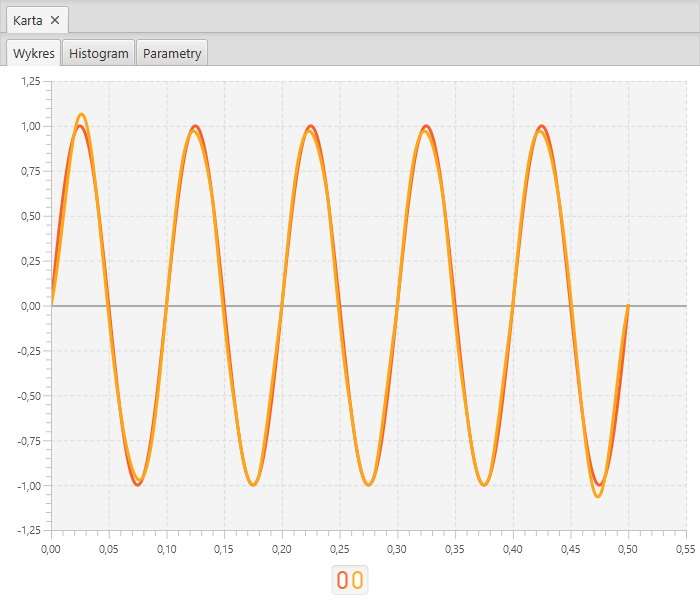
\includegraphics[width=0.8\textwidth]{img/result/experiment4/06/data_draw_original_chart_recon_output_130644.png}
                    \caption{Wykres sygnałów}
                \end{figure}
            }
            \newpage

            \subsubsection{Eksperyment 7} {
                \begin{table}[H]
                    \centering
                    \begin{tabular}{|l|l|l|l|l|}
                        \hline
                        1 & 2 & 3 & 4 & 5   \\ \hline
                        sin & 0.5 & 0.1 & 50 & sinc 25  \\ \hline
                    \end{tabular}
                    \caption{Parametry wejściowe}
                \end{table}

                \begin{table}[H]
                    \centering
                    \begin{tabular}{|l|l|l|l|l|}
                        \hline
                        1 & 2 & 3 & 4   \\ \hline
                        0,0008 & 27,7767 & 31,0143 & 0,1203 \\ \hline
                    \end{tabular}
                    \caption{Parametry wyjściowe}
                \end{table}


                \begin{figure}[H]
                    \centering
                    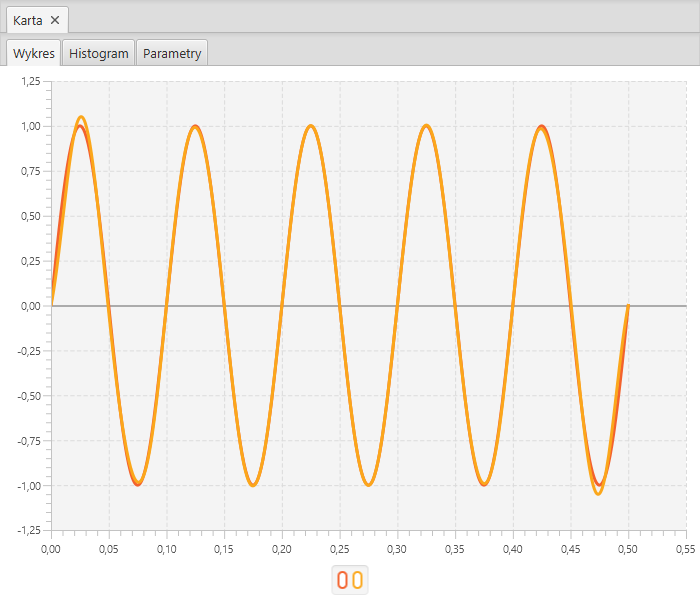
\includegraphics[width=0.8\textwidth]{img/result/experiment4/07/data_draw_original_chart_recon_output_130703.png}
                    \caption{Wykres sygnałów}
                \end{figure}
            }
            \newpage

        }

        \subsection{Badanie kwantyzacji - Wpływ liczby poziomów kwantyzacji sygnału na błąd
        kwantyzacji dla różnych sygnałów} {

            \subsubsection{Eksperyment 1} {
                \begin{table}[H]
                    \centering
                    \begin{tabular}{|l|l|l|l|l|}
                        \hline
                        1 & 2 & 3 & 4 & 5   \\ \hline
                        sin & 1 & 0.25 & 100 & 2      \\ \hline
                    \end{tabular}
                    \caption{Parametry wejściowe}
                \end{table}

                \begin{table}[H]
                    \centering
                    \begin{tabular}{|l|l|l|l|l|l|}
                        \hline
                        1 & 2 & 3 & 4 & 5 & 6  \\ \hline
                        0,227 & 6,4225 & 6,4311 & 0,998 & 7,78 & 0,7745  \\ \hline
                    \end{tabular}
                    \caption{Parametry wyjściowe}
                \end{table}


                \begin{figure}[H]
                    \centering
                    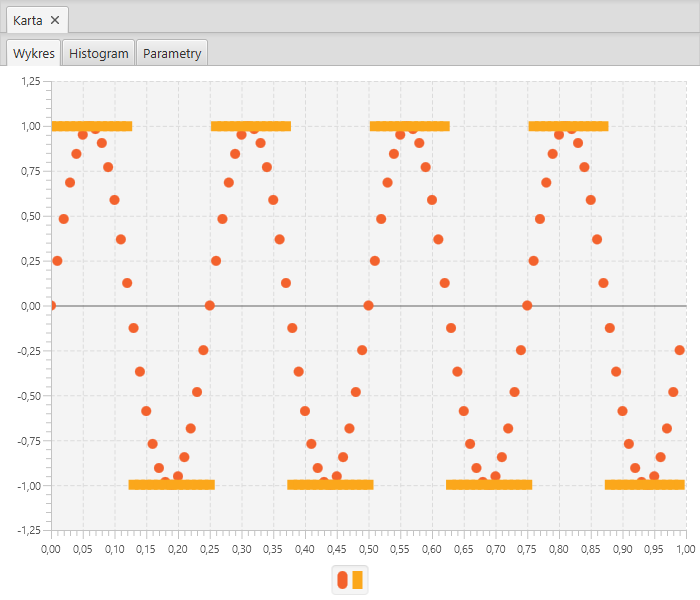
\includegraphics[width=0.8\textwidth]{img/result/experiment5/01/data_draw_sampling_output_quant_output_200408.png}
                    \caption{Wykres sygnałów}
                \end{figure}
            }
            \newpage

            \subsubsection{Eksperyment 2} {
                \begin{table}[H]
                    \centering
                    \begin{tabular}{|l|l|l|l|l|}
                        \hline
                        1 & 2 & 3 & 4 & 5   \\ \hline
                        sin & 1 & 0.25 & 100 & 5    \\ \hline
                    \end{tabular}
                    \caption{Parametry wejściowe}
                \end{table}

                \begin{table}[H]
                    \centering
                    \begin{tabular}{|l|l|l|l|l|l|}
                        \hline
                        1 & 2 & 3 & 4 & 5 & 6  \\ \hline
                        0,0179 & 14,935 & 17,4617 & 0,2487 & 19,82 & 2,1885 \\ \hline
                    \end{tabular}
                    \caption{Parametry wyjściowe}
                \end{table}


                \begin{figure}[H]
                    \centering
                    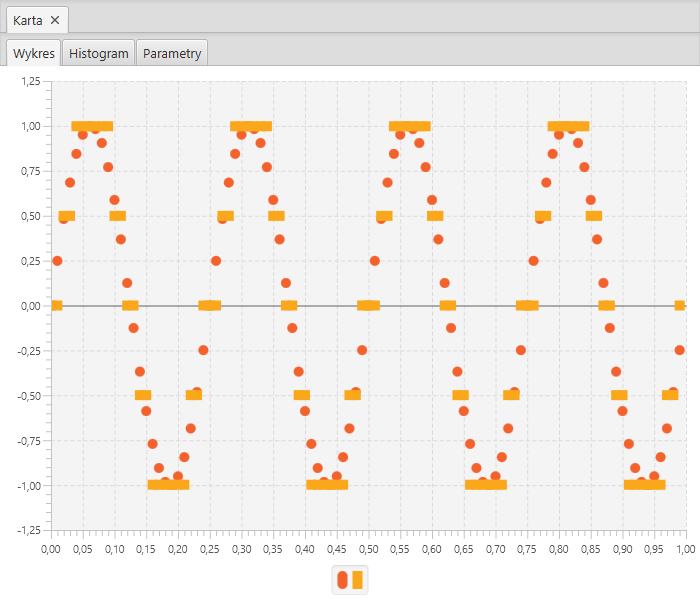
\includegraphics[width=0.8\textwidth]{img/result/experiment5/02/data_draw_sampling_output_quant_output_200417.png}
                    \caption{Wykres sygnałów}
                \end{figure}
            }
            \newpage

            \subsubsection{Eksperyment 3} {
                \begin{table}[H]
                    \centering
                    \begin{tabular}{|l|l|l|l|l|}
                        \hline
                        1 & 2 & 3 & 4 & 5   \\ \hline
                        sin & 1 & 0.25 & 100 & 10    \\ \hline
                    \end{tabular}
                    \caption{Parametry wejściowe}
                \end{table}

                \begin{table}[H]
                    \centering
                    \begin{tabular}{|l|l|l|l|l|l|}
                        \hline
                        1 & 2 & 3 & 4 & 5 & 6  \\ \hline
                        0,0036 & 21,6668 & 24,4014 & 0,1109 & 25,84 & 3,3068 \\ \hline
                    \end{tabular}
                    \caption{Parametry wyjściowe}
                \end{table}


                \begin{figure}[H]
                    \centering
                    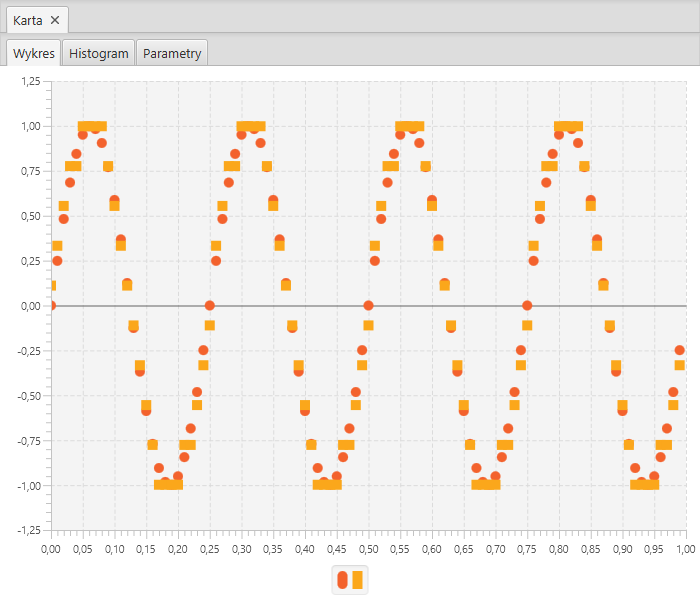
\includegraphics[width=0.8\textwidth]{img/result/experiment5/03/data_draw_sampling_output_quant_output_200425.png}
                    \caption{Wykres sygnałów}
                \end{figure}
            }
            \newpage

            \subsubsection{Eksperyment 4} {
                \begin{table}[H]
                    \centering
                    \begin{tabular}{|l|l|l|l|l|}
                        \hline
                        1 & 2 & 3 & 4 & 5   \\ \hline
                        rect & 1 & 0.25 & 100 & 2  \\ \hline
                    \end{tabular}
                    \caption{Parametry wejściowe}
                \end{table}

                \begin{table}[H]
                    \centering
                    \begin{tabular}{|l|l|l|l|l|l|}
                        \hline
                        1 & 2 & 3 & 4 & 5 & 6  \\ \hline
                        0,0 & inf & inf & 0 & 7,78 & inf \\ \hline
                    \end{tabular}
                    \caption{Parametry wyjściowe}
                \end{table}


                \begin{figure}[H]
                    \centering
                    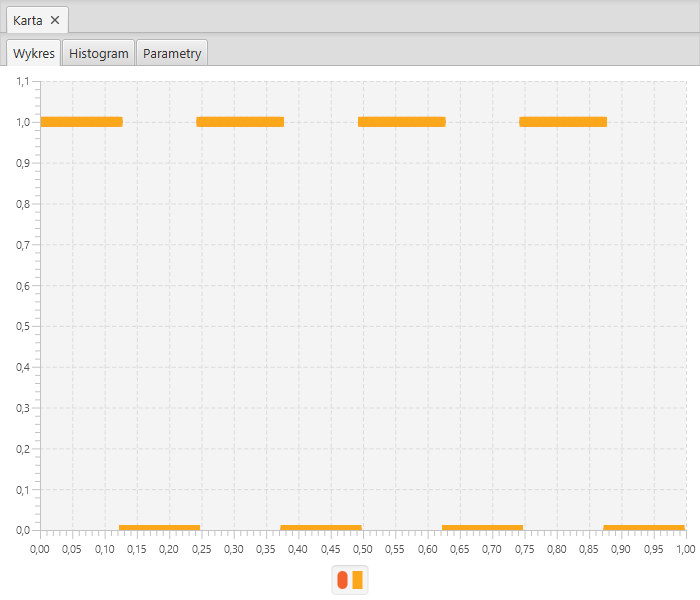
\includegraphics[width=0.8\textwidth]{img/result/experiment5/04/data_draw_sampling_output_quant_output_203951.png}
                    \caption{Wykres sygnałów}
                \end{figure}
            }
            \newpage

            \subsubsection{Eksperyment 5} {
                \begin{table}[H]
                    \centering
                    \begin{tabular}{|l|l|l|l|l|}
                        \hline
                        1 & 2 & 3 & 4 & 5   \\ \hline
                        rect & 1 & 0.25 & 100 & 5  \\ \hline
                    \end{tabular}
                    \caption{Parametry wejściowe}
                \end{table}

                \begin{table}[H]
                    \centering
                    \begin{tabular}{|l|l|l|l|l|l|}
                        \hline
                        1 & 2 & 3 & 4 & 5 & 6  \\ \hline
                        0,0 & inf & inf & 0,0 & 19,82 & inf \\ \hline
                    \end{tabular}
                    \caption{Parametry wyjściowe}
                \end{table}


                \begin{figure}[H]
                    \centering
                    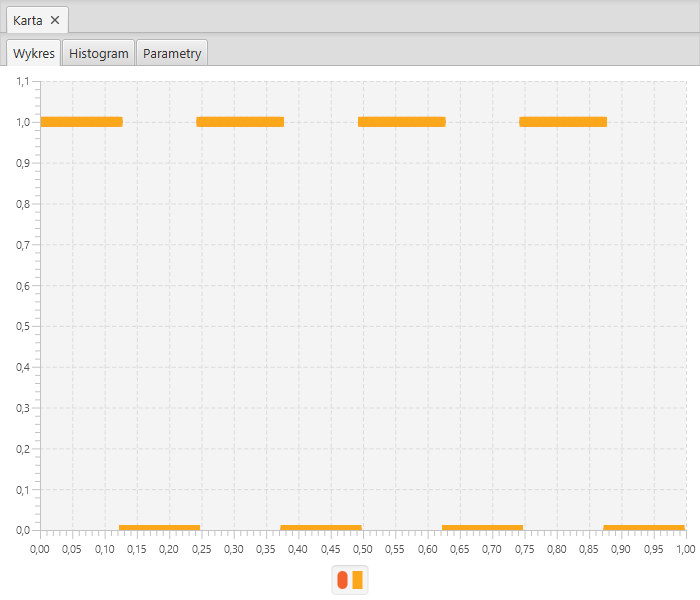
\includegraphics[width=0.8\textwidth]{img/result/experiment5/05/data_draw_sampling_output_quant_output_204002.png}
                    \caption{Wykres sygnałów}
                \end{figure}
            }
            \newpage

            \subsubsection{Eksperyment 6} {
                \begin{table}[H]
                    \centering
                    \begin{tabular}{|l|l|l|l|l|}
                        \hline
                        1 & 2 & 3 & 4 & 5   \\ \hline
                        triang & 1 & 0.25 & 100 & 2   \\ \hline
                    \end{tabular}
                    \caption{Parametry wejściowe}
                \end{table}

                \begin{table}[H]
                    \centering
                    \begin{tabular}{|l|l|l|l|l|l|}
                        \hline
                        1 & 2 & 3 & 4 & 5 & 6  \\ \hline
                        0,0748 & 8,2331 & 11,0865 & 0,48 & 7,78 & 1,0753 \\ \hline
                    \end{tabular}
                    \caption{Parametry wyjściowe}
                \end{table}


                \begin{figure}[H]
                    \centering
                    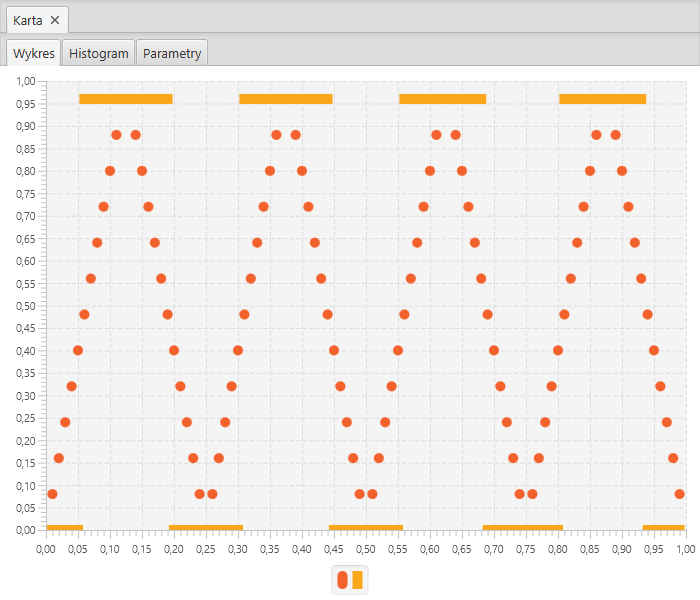
\includegraphics[width=0.8\textwidth]{img/result/experiment5/06/data_draw_sampling_output_quant_output_202217.png}
                    \caption{Wykres sygnałów}
                \end{figure}
            }
            \newpage

            \subsubsection{Eksperyment 7} {
                \begin{table}[H]
                    \centering
                    \begin{tabular}{|l|l|l|l|l|}
                        \hline
                        1 & 2 & 3 & 4 & 5   \\ \hline
                        triang & 1 & 0.25 & 100 & 3   \\ \hline
                    \end{tabular}
                    \caption{Parametry wejściowe}
                \end{table}

                \begin{table}[H]
                    \centering
                    \begin{tabular}{|l|l|l|l|l|l|}
                        \hline
                        1 & 2 & 3 & 4 & 5 & 6  \\ \hline
                        0,0195 & 12,7755 & 16,9322 & 0,24 & 13,8 & 1,8298 \\ \hline
                    \end{tabular}
                    \caption{Parametry wyjściowe}
                \end{table}


                \begin{figure}[H]
                    \centering
                    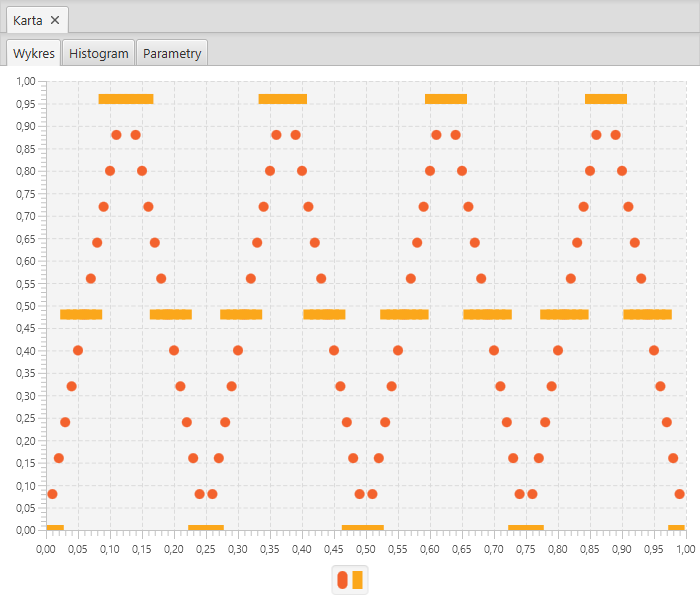
\includegraphics[width=0.8\textwidth]{img/result/experiment5/07/data_draw_sampling_output_quant_output_202228.png}
                    \caption{Wykres sygnałów}
                \end{figure}
            }
            \newpage

            \subsubsection{Eksperyment 8} {
                \begin{table}[H]
                    \centering
                    \begin{tabular}{|l|l|l|l|l|}
                        \hline
                        1 & 2 & 3 & 4 & 5   \\ \hline
                        triang & 1 & 0.25 & 100 & 5  \\ \hline
                    \end{tabular}
                    \caption{Parametry wejściowe}
                \end{table}

                \begin{table}[H]
                    \centering
                    \begin{tabular}{|l|l|l|l|l|l|}
                        \hline
                        1 & 2 & 3 & 4 & 5 & 6  \\ \hline
                        0,0041 & 19,2038 & 23,6991 & 0,08 & 19,82 & 2,8976 \\ \hline
                    \end{tabular}
                    \caption{Parametry wyjściowe}
                \end{table}


                \begin{figure}[H]
                    \centering
                    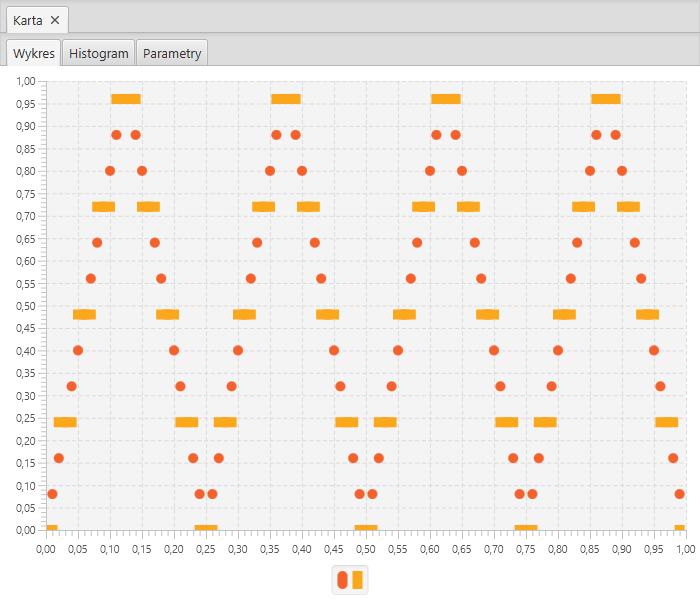
\includegraphics[width=0.8\textwidth]{img/result/experiment5/08/data_draw_sampling_output_quant_output_202238.png}
                    \caption{Wykres sygnałów}
                \end{figure}
            }
            \newpage

        }

    }
%--------------------------------------------------------------------------------------%
    \section{Dyskusja} {

        \subsection{Badanie jakości rekonstrukcji sygnału - Wpływ zależności między częstotliwością
        sygnału a częstotliwością próbkowania na jakość rekonstrukcji dla jej różnych rodzajów} {

            Pierwsza seria eksperymentów bada jak na jakość rekonstrukcji sygnał różnymi metodami wpływa
            stosunek częstotliwości sygnału do częstotliwości próbkowania. Rozważamy w tym przypadku oczywiście
            sygnały okresowe. We wszystkich eksperymentach generowany został sygnał \emph{sinus} o
            częstotliwości $10Hz$ trwający przez $0.5s$. Zmianie ulegała metoda rekonstrukcji i czestotliwość
            próbkowania. Ta ostatnia przyjmowała zawsze wartości przynajmniej dwa razy większe od częstotliwości
            sygnału aby zapobiec występowaniu zjawiska aliasingu, które zostanie omówione później.

            Po przeanalizowaniu wyników eksperymentów od 1 do 4, w których wykorzystano metodę roknstrukcji
            opartą o funkcję \emph{sinc}, widzimy utrzymującą się następującą zależność: wraz ze wzrostem
            częstotliwości próbkowania zwiększa się jakość rekonstrukcji sygnału. Widać to po malejących
            wartościach parametrów SNR i MD a rosnących wartościach parametrów SNR i PSNR. Co ciekawe, jakość ta
            poprawiła się co najmniej kilkadziesiąt razy przy zmianie częstotliwości próbkowania z $21Hz$ na
            $30Hz$, późniejsze różnice w jakości rekonstrukcji są znacznie mniejsze - jakość zwiększa się kilka
            razy (rozpatrując zwłaszcza błąd średniokwadratowy). Ten sam wniosek można wysnuć na podstawie
            wizualnej oceny wykresów, widać na nich, że czym częstotliwości próbkowania bliższe są dwukrotności
            częstotliwości sygnału tym większe różnice w jakości rekonstrukcji. W pewnym momencie zmiana
            częstotliwości próbkowania stanie się pomijalnie mała. Oczywiście należy pamiętać, że wpływ na
            jakość rekonstrukcji ma także liczba próbek i tym samym czas trwania przetwarzanego sygnału.

            Eksperymenty 5 do 7 prezentują proces rekonstrukcji za pomocą ekstrapolacji zerowego rzędu. Funkcja
            zrekonstruowana będzie się składać z wielu funkcji stałych. Zarówno po wynikach jak i po wykresach
            widać, że metoda ta sprawdza się znacznie gorzej niż metoda omawiana poprzednio. Ekstrapolacja
            zerowego rzędu nie nadaje się do rekonstrukcji funkcji sin. Oczywiście, zgodnie z intuicją, również
            jakość tej rekonstrukcji będzie się poprawiać wraz ze zwiększeniem częstotliwości próbkowania,
            jednak należy zauważyć, że poprawy te są mniejsze, niż w przypadku wykorzystania funkcji
            \emph{sinc}.

            Ostatnią wykorzystaną metodą rekonstrukcji jest interpolacja pierwszego rzędu. Do przybliżenia
            wykorzystujemy tutaj funkcje liniowe. Od razu widać, że sprawdzają się one lepiej niż funkcje stałe
            (przy ekstrapolacji zerowego rzędu), dalej jednak wyniki pozostają znacznie gorsze niż w przypadku
            pierwszej omawianej metody. Co ciekawe, po wynikach eksperymentu 10 można zacząć oczekiwać, że przy
            odpowiedniej liczbie próbek uda się osiągnąć za pomocą interpolacji pierwszego rzędu wyniki podobnej
            jakości jak za pomocą funkcji \emph{sinc}.

    }


        \subsection{Badanie jakości rekonstrukcji sygnału - Wpływ rodzaju sygnału na jakość
        rekonstrukcji dla jej różnych rodzajów} {

        W drugiej przeprowadzonej serii eksperymentów zbadany został wpływ rodzaju sygnału na jakoś
        rekonstrukcji i tutaj również wzięto pod rozwagę różne jej metody. Zbadane zostały trzy różne
        sygnały okresowe: sinus, sygnał prostokątny i sygnał trójkątny. Dla każdego z nich zastosowano
        wszystkie omówione wcześniej metody rekonstrukcji.

        Eksperymenty 1 - 3 skupiają się na działaniu metody rekonstrukcji opartej o funkcję \emph{sinc}.
        Widzimy tutaj to, co już zostało spostrzeżone wcześniej, a mianowicie, że ta metoda bardzo dobrze
        sprawdza się przy rekonstrukcji funkcji sinus (i tym samym funkcji będących pewną sumą funkcji
        sinus). Eksperyment 2 pokazuje, że funkcja \emph{sinc} niespecjalnie nadaje się do rekonstrukcji
        funkcji kwadratowej, co jest również zgodne z intuicją. Trochę lepiej (dokładnie rzecz ujmując kilka
        razy lepiej) sprawdza się natomiast do rekonstrukcji funkcji trójkątnej.

        W doświadczeniu 4 z tej serii widzimy wykorzystanie ekstrapolacji zerowego rzędu do rekonstrukcji
        funkcji sinus. Stwierdzamy to co zostało stwierdzone już wcześniej, metoda ta nie pasuje do tego
        rodzaju funkcji. Ciekawe wyniki natomiast prezentuje doświadczenie kolejne, w którym do
        rekonstrukcji funkcji kwadratowej wykorzystano właściwie funkcję kwadratową. Jest to bardzo
        specyficzna sytuacja i można by pomyśleć, że taka rekonstrukcja sprawdzi się dobrze. Ocena wizualna
        wypada dosyć pomyślnie natomiast wyniki wskazują na to, że jest to rekonstrukcja niewiele lepsza
        (prawie dwa razy) niż rekonstrukcja sinusa. Wynika to z faktu, że jeżeli już pojawiają się różnice
        między sygnałem oryginalnym a zrekonstruowanym to zawsze są one bardzo duże (równe wartości
        amplitudy). Mechanizm taki prowadzi do dużego błędu średniokwadratowego i słabego stosunku
        sygnał-szum. Maksymalna różnica w oczywisty sposób wynosi 1. Warto porównać ten eksperyment z
        eksperymentem 2 aby zobaczyć, że jakoś rekonstrukcji rzeczywiście jest gorsza, niż z wykorzystaniem
        funkcji \emph{sinc}. Aby poprawić jakość takiej rekonstrukcji należałoby oczywiście zwiększyć
        znacznie częstotliwość próbkowania i wtedy prawdopodobnie uzyskałoby się wyniki znacznie lepsze niż
        przy rekonstrukcji funkcji kwadratowej metodą \emph{sinc}. Doświadczenie 6 przedstawia rekonstrukcję
        funkcji trójkątnej i podobnie jak rekonstrukcja funkcji sinus nie wypada ona zbyt pomyślnie, choć co
        ciekawe, wciąż lepiej niż w doświadczeniu poprzednim.

        Ostatnia grupa doświadczeń z serii drugiej dotyczy rekonstrukcji interpolacją pierwszego rzędu.
        Doświadczenie 7 potwierdza to co już wiadome, że rekonstrukcja funkcji sin tą metodą daje wyniki
        gorsze niż metodą opartą o funkcję \emph{sinc} ale lepsze niż z wykorzsstaniem ekstrapolacji
        zerowego rzędu. Najciekawsze wnioski można wyciągnąć na postawie doświadczeń 8 i 9. Widać tutaj, że
        ta metoda sprawdza się najlepiej spośród wszystkich omawianych metod, do rekonstrukcji funkcji
        kwadratowej. Jest to wyraźnie widoczne i pozostaje ciekawym wnioskiem, że ta metoda działa lepiej
        niż ekstrapolacja zerowego rzędu, która wizualnie lepiej pasuje do funkcji kwadratowej. Jeżeli
        chodzi o funkcję trójkątną to błąd średniokwadratowy nie niesie tutaj wyraźnej informacji o
        przewadze tej metody (wynika to ze zbyt małej częstotliwości próbkowania) nad ekstrapolacją zerowego
        rzędu. Natomiast dopiero stosunek sygnał-szum daje jasny obraz na jakość rekonstrukcji tego sygnału
        i pozwala stwierdzić, że jest ona zaledwie nieznacznie gorsza niż z wykorzystaniem funkcji
        \emph{sinc}, natomiast znacznie lepsza (ponad dwa razy) niż ekstrapolacja zerowego rzędu.

        }


        \subsection{Badanie jakości rekonstrukcji sygnału - Zjawisko aliasingu} {

        W trzeciej serii eksperymentów zostało zaprezentowane zjawisko aliasingu. Wykonano trzy
        eksperymenty. W każdym z nich częstotliwośc wygenerowanego sygnału (sinus) znacznie przekraczała
        częstotliwość Nyquista (połowę częstotliwości próbkowania) i dochodziło do wzmocnienia (pojawienia
        się) pewnej częstotliwości w paśmie użytecznym. Aby powstała ta nowa częstotliwość $f_0$
        częstotliwość sygnału $f_d$ zostanie ustawiona na $f_d = k \cdot f_s + f_0$, gdzie $f_s$ to
        częstotliwość próbkowania a k to pewna liczba całkowita.

        W eksperymencie pierwszym częstotliwość sygnału wynosi $7Hz = 1 \cdot 5Hz + 2Hz$, powstała
        częstotliwość $f_0 = 2Hz$. Zjawisko to zostało przedstawione na wykresie, faktycznie okazuje się, że
        sygnał powstały po zrekonstruowaniu wyników próbkowania ma częstotliwość $2Hz$. Analogicznie w
        doświadczeniu 2 częstotliwość $f_d$ została ustawiona na 12 Hz co znowu daje $f_0 = 2Hz$ i jest
        zgodne z wykresem. Ostatnie doświadczenie z tej serii prezentuje powstanie częstotliwości $f_0 =
        1Hz$ w wyniku ustawienia częstotliwości sygnału $f_d$ na 11Hz.

        }


        \subsection{Badanie jakości rekonstrukcji sygnału - Wpływ wartości N na jakość
        rekonstrukcji przy wykorzystaniu metody sinc} {

        Dotychczas przy przeprowadzaniu rekonstrukcji z wykorzystaniem funkcji \emph{sinc} jej parametr $N$
        zawsze był ustawion na 100. Nie zajmowaliśmy się bowiem badaniem jego wpływu na jakość
        rekonstrukcji. Był on więc na tyle duży, aby zapewnić jak najlepsze wyniki działania tej metody. Ta
        seria eksperymentów ma na celu zbadać właśnie jakość rekonstrukcji sygnału metodą opartą o funkcję
        \emph{sin} przy różnych wartościach jej parametru $N$. Wykonano 7 eksperymentów a wartość $N$
        zmieniała się od 1 aż do 25. Zarówno po wykresach jak i wynikach porównania sygnału początkowego z
        sygnałem zrekonstruowanym widać, że na samym początku, dla wartości 1 i 2, rekonstrukcja jest bardzo
        niedokładna. Natomiast już przy wartości 3 poprawia się ona wielokrotnie. Później ulega już
        niewielkim zmianom, przez chwilę niecznacznie rośnia a póżniej zmienia się już w różnych kierunkach,
        mieści się jednak w jakimś stałym zakresie wartości.

        }

        \subsection{Badanie kwantyzacji - Wpływ liczby poziomów kwantyzacji sygnału na błąd
        kwantyzacji dla różnych sygnałów} {
        Ostatnia seria eksperymentów została poświęcona
        badaniu błędu powstałego w wyniku kwantyzacji.
        Zbadane zostały trzy różne sygnały, podobnie jak
        w poprzednich doświadczeniach - sinus, funkcja
        prostokątna i funkcja trójkątna. Dla każdego z
        nich zastosowano różne liczby poziomów
        kwantyzacji.

        Tym razem najpierw zastanowimy się nad wynikami
        kwantyzacji spróbkowanej funkcji prostokątnej.
        Wyniki te są inne od pozostałych i badzo
        specyficzne, ze względu na to, że funkcja
        prostokątna jest właściwie ze swojej definicji
        już skwantyzowana. Przyjmuje bowiem jedynie dwie
        różne wartości. Wynik kwantyzacji dla dwóch lub
        więce poziomów będzie się więc zawsze pokrywał z
        wynikiem próbkowania. Na wykresach z
        eksperymentów 4 i 5 widać jedynie wynik
        kwantyzacji, gdyż zakrywa on całkowicie funkcję
        oryginalną. Ponadto wynik porównania, zwłaszcza
        wartości \emph{inf} dla stosunku sygnał-szum
        potwierdzają, że oba porównywane sygnały są
        takie same.

        Doświadczenia od 1 do 3 przedstawiają proces
        kwantyzacji spróbkowanej funkcji sinus. Za
        pierwszym razem poziomy są dwa, za drugim 5 a za
        trzecim 10. Z każdym kolejnym wynikiem błąd
        średniokwadratowy maleje a stosunek sygnał-szum
        rośnie, oczywistym wnioskiem jest więc, że wraz
        ze wzrostem liczby poziomów kwantyzacji błąd
        kwantyzacji maleje. Dokładnie ten sam wniosek
        można wysnuć na podstawie eksperymentów 6, 7 i
        8. Na których badana jest funkcja trójkątna.

        Warto jeszcze zastanowić się chwilę nad
        porównaniem otrzymanych wartości SNR z
        wartościami teoretycznymi dla sygnału
        sinusoidalnego dla idealnego przetwornika A/C.
        We wszystkich trzech doświadczeniach widać, że
        wartości te są zbliżone, dokładnie rzecz ujmując
        nie osiągnięto tak dużego stosunku sygnał-szum
        jak wartość teoretyczna. Jednak wynika to
        prawdopodobnie z liczby rozważanych próbek i
        częstotliwości próbkowania.
        }

    }

        \section{Wnioski} {

        \begin{itemize}
        \item Zwiększenie częstotliwości próbkowania w stosunku do częstotliwości sygnału ma
        pozytywny wpływ na jakość rekonstrukcji
        \item Największy wzrost jakości rekonstrukcji przy zwiększaniu częstotliwości
        próbkowania występuje w ich początkowym przedziale
        \item Do rekonstrukcji funkcji sinus najlepiej sprawdza się metoda oparta o funkcję
        \emph{sinc} a najgorzej ekstrapolacja zerowego rzędu
        \item Do rekonstrukcji funkcji kwadratowej najlepiej sprawdza się interpolacja
        pierwszego rzędu
        \item Do rekonstrukcji funkcji trójkątnej sprawdza się dobrze zarówno metoda oparta o
        funkcję \emph{sinc} jak i interpolacja pierwszego rzędu
        \item Błąd średniokwadratowy nie zawsze jest wystarczającą miarą do stwierdzenia różnic
        w jakości rekonstrukcji różnymi metodami
        \item Jeżeli częstotliwość sygnału jest większa od połowy częstotliwości próbkowania
        zachodzi zjawisko \emph{aliasingu}
        \item Parametr $N$ w metodzie rekonstrukcji opartej o funkcję \emph{sinc} ma decydujące
        znacznie dla jakości rekonstrukcji. Przy najmniejszych wartościach (1 lub kilka)
        jego zwiększanie poprawia jakość natomiast od pewnego momentu jego zmiany nie mają
        zbytniego znaczenia.
        \item Błąd kwantyzacji maleje wraz ze wzrostem
        liczby poziomów kwantyzacji
        \end{itemize}
        }
%--------------------------------------------------------------------------------------%
\renewcommand\refname{Bibliografia}
\bibliographystyle{plain}
\bibliography{bibliografia_wzor}

\end{document}
